\documentclass[journal]{IEEEtran}
\usepackage{amsmath,amssymb,amsfonts}
\usepackage{graphicx}
\usepackage{booktabs}
\usepackage{multirow}
\usepackage{array}
\usepackage{textcase}
\usepackage{url}
\usepackage{textcomp}
\usepackage{hyperref}
\usepackage[table]{xcolor}
\usepackage{tikz-cd}
\usepackage{tikz}
\usetikzlibrary{shapes.geometric, shapes.misc, arrows.meta, positioning, calc}
\usepackage{pgfplots}
\usepackage{pgfplotstable}
\pgfplotsset{compat=1.18}
\usepgfplotslibrary{groupplots}


\begin{document}
\raggedbottom
\setlength{\emergencystretch}{1.5em}
\hbadness=10000

\title{An Explainable Physics-Guided Digital Twin for Multi-Horizon Glucose Forecasting in Type 1 Diabetes}

\author{
\IEEEauthorblockN{Samyak Jain, Dhriti Goswami, Yugananda Malhotra}\\
\IEEEauthorblockA{
Bharati Vidyapeeth's College of Engineering New Delhi, 110063, India\\
sammyyakk@gmail.com; goswami.dhritid@gmail.com; yugnanda\_malhotra@yahoo.com
}
}


\maketitle

\begin{abstract}
\textbf{Background and objective:} Glucose dynamics in type 1 diabetes (T1D) are nonlinear, delayed, and patient-specific, influenced by meals and insulin. Clinically meaningful forecasting requires valid prediction horizons and comparison with persistence baselines. This study proposes an explainable, physics-guided digital twin integrating deep sequence learning with mechanistic physiological modeling for personalized, multi-horizon glucose forecasting.

\textbf{Methods:} A gap-aware pipeline was developed using the OhioT1DM dataset, ensuring accurate horizon-specific glucose targets. The model combines a compact Transformer encoder with a differentiable Bergman Minimal Model, extended with subcutaneous insulin and gut absorption states, patient-specific parameter estimation, and a non-crossing quantile head for uncertainty. Twelve subjects and 26,498 test windows were evaluated under personalized and subject-disjoint leave-one-subject-out (LOSO) protocols. Performance was assessed across 30–120-minute horizons using RMSE, skill over persistence, Clarke/Parkes error distributions, hypoglycemia-alarm sensitivity, and feature attribution.

\textbf{Results:} Across all 12 subjects, the model achieved RMSE values of 18.84, 30.52, 38.60, and 44.46 mg/dL at 30, 60, 90, and 120 minutes, respectively, with a 19.4-21.2\% improvement over persistence. LOSO validation confirmed the personalization while the physics constraints preserved accuracy and enabled estimation of patient-specific insulin sensitivity. The lower-quantile alarm further improved hypoglycemia sensitivity.

\textbf{Conclusion:} Physiological constraints with AI-based forecasting support personalized diabetes monitoring. The proposed framework demonstrates potential for clinical translation through stable insulin sensitivity estimation and improved hypoglycemia prediction, while supporting interpretable,physics-guided forecasting.
\end{abstract}

\begin{IEEEkeywords}
continuous glucose monitoring, digital twin, type 1 diabetes, physics-informed learning, Transformer, uncertainty quantification, explainable artificial intelligence
\end{IEEEkeywords}

%=================================================================
\section{Introduction}

\subsection{Background}

Type 1 diabetes (T1D) is a disease involving the immune-mediated destruction pancreatic $\beta$-cells and thus individuals with type 1 diabetes require lifelong exogenous insulin replacement and glucose monitoring, disease-specific education, diet, and lifestyle modification remain cornerstones of its management alongside insulin therapy. Glucose-insulin dynamics, however, are governed by nonlinear, patient-specific physiology, as described mechanistically through the Bergman Minimal Model~\cite{ref1}. Despite advancements in continuous glucose monitoring (CGM) hardware, it remains very difficult to build a system that converts raw diabetes data into personalized, actionable medical recommendations~\cite{ref2}.

This has driven the development of machine-learning approaches for CGM forecasting progressing from black-box sequence models, including recurrent networks to attention-based Transformer architectures
[\hyperref[ref3label]{3}-\hyperref[ref4label]{4}]which can achieve strong short-horizon accuracy but function as black boxes offering clinicians little interpretability~\cite{ref3,ref5}. This limitation motivated a shift toward increasingly physiology-aware approaches that fold a physics-consistency penalty derived from mechanistic models, following the Physics-Informed Neural Network (PINN) paradigm~[\hyperref[ref6label]{6}-\hyperref[ref10label]{10}]. However, validation has typically remained simulator-only or narrowly dataset-specific~[\hyperref[ref7label]{7}-\hyperref[ref8label]{8}]. More recent systems introduced patient-specific digital twins and prospective evaluation~[\hyperref[ref11label]{11}-\hyperref[ref13label]{13}]. Yet translating predictions into safe, actionable recommendations remains challenging, with reinforcement-learning approaches still considered insufficiently clinically safe~\cite{ref14}.

The field has therefore advanced along several parallel tracks;interpretable risk prediction, physiology-constrained forecasting, digital-twin construction and validation, and increasingly capable sequence-modelling backbones that remain largely disconnected from one another.

\subsection{Literature Review}

Systematic reviews of Type 1 diabetes digital twins note that existing systems are not yet comprehensive, multi-scale virtual replicas, and most model glucose-insulin metabolism in isolation rather than the full patient~\cite{ref2}, motivating a more integrated, personalized digital twin.

A natural first step was showing CGM-based risk prediction could be both accurate and interpretable. Explainable short-horizon hypoglycemia/hyperglycemia prediction models added SHAP-based feature attributions to opaque risk classifiers, demonstrating strong, interpretable patient-level forecasting~\cite{ref3}. This explained \emph{why} a risk was predicted but not what to do about it, motivating subsequent work using SHAP attributions to guide bounded, one-step behavioural recommendations on OhioT1DM~\cite{ref6}. However, the approach remained exploratory and was not considered clinically safe, shifting subsequent focus toward postprandial glucose response. Explainable postprandial glucose modeling attributed meal-response forecasts to specific inputs, achieving personalized, transparent prediction~\cite{ref7}, though remaining purely data-driven with no physiological constraint.

Next, physiology was embedded directly into the learning objective. Early PINN-based glucose predictors added a physics-consistency penalty to sequence learning, improving short-term in-silico prediction while preserving mechanistic plausibility, though validation stayed simulator-only~\cite{ref9}. Bergman-constrained PINN models tied the network explicitly to the Bergman Minimal Model, improving physiological plausibility on real T1DM data, though evaluation remained narrow and dataset-specific~\cite{ref10}. Hybrid physiology and deep learning architectures embedded glucose--insulin dynamics into both architecture and training, achieving reliable predictions under limited real-subject data, but remained forecasting models rather than virtual patients~\cite{ref11}. Physics-guided sequence models addressed recurrent black-box models' inability to distinguish meal and insulin effects via physics-LSTM hybrids, bridging sequence modeling and physiology-guided forecasting, still without a full virtual-patient representation~\cite{ref12}.

By integrating physiology-based models with LSTM learning, it produced patient-specific virtual subjects for in-silico therapy testing, moving from forecasting toward simulation, though remaining a research framework rather than a clinically validated system~\cite{ref13}. An open-source digital-twin methodology addressed this by identifying a personalized glucose-insulin model directly from routine CGM, insulin, and meal data, showing non-invasive, CGM-only twinning suffices for personalized counterfactual simulation, though use remained mainly retrospective~\cite{ref14}. Simulation-to-reality data augmentation then used simulated patients as synthetic data generators to offset limited T1D data availability, improving glucose prediction model training without yet proving twins support decision-making~\cite{ref15}. Twin fidelity was addressed by validating physiologically constrained digital twins against real exercise data from 394 cases -- strong evidence simulated twins match observed clinical dynamics, though still simulation-centric~\cite{ref16}. This gap was partly closed by a randomized clinical trial of a twin-enhanced decision-support system, showing improved time-in-range and reduced hypoglycaemia within a bolus-dosing-centered system~\cite{ref17}, further extended to full adaptive biobehavioural co-adaptation for automated insulin delivery (AID) in a six-month randomized trial, where each participant's AID data generated a cloud-based digital twin biweekly re-optimizing therapy parameters, overcoming the typical time-in-range plateau -- though optimizing therapy periodically rather than forecasting glucose continuously in real time~\cite{ref18}.

In parallel, attention-based Transformer forecasting on OhioT1DM outperformed classical machine-learning baselines (XGBoost, 1D-CNN) for short-horizon prediction but remained a plain sequence model with limited interpretability~\cite{ref19}, extended to interpretable multi-horizon forecasting with attention over temporal and static covariates, though without benchmarking against an explicit recurrent-hybrid baseline~\cite{ref20}. A hybrid Transformer-LSTM architecture addressed pure attention models' under-modeling of short-term fluctuations, improving short/medium-horizon accuracy, though horizon coverage stopped short of 120 minutes~\cite{ref21}. Long-horizon hybrid Transformer-LSTM models pushed prediction to 120 minutes with richer clinical inputs and strong safety-zone performance, but remained purely data-driven~\cite{ref22}. Metadata-aware personalization improved individualized forecasting via physiological signals, demographics, and device metadata, but required centralized pooling of sensitive data~\cite{ref23}, addressed by personalized federated learning training models across sites without centralizing data, focused on high-risk glycaemic-excursion regions, though not addressing on-device efficiency or interpretability~\cite{ref24}. Practical deployability was addressed via lightweight, edge-deployable Transformer models, still lacking native uncertainty quantification or interpretability~\cite{ref25}. A Temporal Fusion Transformer with built-in attention-based feature/temporal importance and calibrated predictive uncertainty addressed this directly, outperforming prior baselines by $\geq$13\% RMSE, though attention weights weren't validated against physiological ground truth~\cite{ref26}. Self-supervised Transformer pretraining produced reusable glucose representations supporting multiple downstream tasks (screening, dietary prediction), but lacked grounding in verified clinical guidelines~\cite{ref27}, addressed by a retrieval-augmented generation framework for diabetes education, retrieving verified medical content before generation to reduce hallucination and improve response accuracy, though applied to conversational education rather than numerical forecasting~\cite{ref28}. Most recently, retrieval-augmented forecasting applied this contextualization directly to CGM prediction, drawing on similar historical episodes rather than raw sequences alone, but still requiring mechanistic grounding, SHAP-style explanation, and prospective clinical validation~\cite{ref29}.

Table~\ref{tab:landscape} situates this study among OhioT1DM forecasting approaches, grouped into physics-informed, non-physics learned/statistical, physics-informed LSTM, and physics-informed hybrid architectures, with the proposed method in the latter category.

\begin{table*}[t]
\centering
\caption{Landscape comparison of OhioT1DM blood-glucose forecasting studies by architecture family (30/60/90/120-minute horizons)}
\label{tab:landscape}
\tiny
\resizebox{\textwidth}{!}{%
\begin{tabular}{l>{\raggedright\arraybackslash}p{2.6cm}rrrrrrrr}
\toprule
Reference & Methodology & RMSE@30 & MAE@30 & RMSE@60 & MAE@60 & RMSE@90 & MAE@90 & RMSE@120 & MAE@120 \\
\midrule
\multicolumn{10}{l}{\textit{Non-physics learned/statistical sequence models (6 subjects, official split)}} \\
\cite{ref66} & Stacked regression + activity & 18.99 & 13.73 & 33.39 & 25.04 & \multicolumn{2}{c}{not reported$^{\dagger}$} & \multicolumn{2}{c}{not reported$^{\dagger}$} \\
\cite{ref67} & Multi-lag stacking & 19.21 & 13.93 & 33.65 & 25.31 & \multicolumn{2}{c}{not reported$^{\dagger}$} & \multicolumn{2}{c}{not reported$^{\dagger}$} \\
\cite{ref68} & Latent-variable statistical & 19.37 & 13.76 & 32.59 & 24.64 & \multicolumn{2}{c}{not reported$^{\dagger}$} & \multicolumn{2}{c}{not reported$^{\dagger}$} \\
\cite{ref69} & Multi-class LSTM (+2018 data) & 19.40 & 13.90 & 33.40 & 25.00 & \multicolumn{2}{c}{not reported$^{\dagger}$} & \multicolumn{2}{c}{not reported$^{\dagger}$} \\
\cite{ref71} & Multitask CRNN & 19.79 & 13.62 & 33.73 & 24.54 & \multicolumn{2}{c}{not reported$^{\dagger}$} & \multicolumn{2}{c}{not reported$^{\dagger}$} \\
\cite{ref69} & Multi-class LSTM & 19.80 & 14.40 & 34.00 & 25.80 & \multicolumn{2}{c}{not reported$^{\dagger}$} & \multicolumn{2}{c}{not reported$^{\dagger}$} \\
\cite{ref72} & Online ARMA + residual net & 20.03 & 14.52 & 34.89 & 24.61 & \multicolumn{2}{c}{not reported$^{\dagger}$} & \multicolumn{2}{c}{not reported$^{\dagger}$} \\
\cite{ref73} & Personalised interpretable LSTM & 20.20 & 14.74 & 34.19 & 25.98 & \multicolumn{2}{c}{not reported$^{\dagger}$} & \multicolumn{2}{c}{not reported$^{\dagger}$} \\
\cite{ref71} & Single-task CRNN (ablation) & 20.67 & 14.28 & 34.40 & 24.67 & \multicolumn{2}{c}{not reported$^{\dagger}$} & \multicolumn{2}{c}{not reported$^{\dagger}$} \\
\cite{ref74} & Seq2Seq BiLSTM & 21.80 & 15.00 & 35.00 & 25.00 & \multicolumn{2}{c}{not reported$^{\dagger}$} & \multicolumn{2}{c}{not reported$^{\dagger}$} \\
\midrule
\multicolumn{10}{l}{\textit{Physics-informed + other-architecture hybrid (6 subjects, official split)$^{\dagger}$}} \\
\cite{ref58} & Physiological model + ANN & 19.33 & -- & 31.72 & -- & \multicolumn{2}{c}{not reported$^{\dagger}$} & \multicolumn{2}{c}{not reported$^{\dagger}$} \\
\midrule
-- & \textbf{Current Work: Physics-guided PINN (Bergman) + Transformer} & \textbf{18.74} & \textbf{13.24} & \textbf{31.16} & \textbf{22.55} & \textbf{39.52} & \textbf{29.14} & \textbf{45.39} & \textbf{34.03} \\
-- & \emph{Persistence baseline (ours)} & 24.22 & 17.45 & 40.11 & 29.51 & 51.15 & 38.34 & 58.98 & 44.83 \\
\bottomrule
\end{tabular}%
}
\vspace{2pt}
\raggedright\footnotesize
$^{\dagger}$ All listed studies use the 2020 six-subject official-split cohort except \cite{ref58}, which uses the 2018 six-subject official-split cohort; values are not directly comparable across cohorts. The 90- and 120-minute entries marked ``not reported'' reflect the absence of protocol-matched published OhioT1DM values; the BGLP challenges required only 30- and 60-minute forecasts. The current work's 90- and 120-minute figures use the same matched six-subject subset as its 30- and 60-minute columns. Table~\ref{tab:official} reports the all-subject results against the corresponding persistence baseline.
\end{table*}
 


\subsection{Objectives}
\begin{itemize}
\sloppy
\item To develop a physics-guided digital twin that couples a Transformer forecaster with Bergman Minimal Model constraints, delivering 30,60,90,120 minute glucose forecasts that consistently outperform persistence.
\item To estimate patient-specific insulin sensitivity from routine CGM, insulin, and meal data, and to verify that it is individual, stable, and consistent with total daily insulin dose under personalized evaluation.
\item To quantify forecast uncertainty and improve hypoglycemia detection through calibrated lower-quantile alarms.
\item To support interpretation of predictions through integrated-gradients attributions cross-checked with permutation importance, and to validate the framework on real OhioT1DM data under both personalized and subject-disjoint (leave-one-subject-out) protocols.
\end{itemize}

The paper is structured as follows. Section~I introduces the background, related literature, and objectives. Section~II details the methodology, including data acquisition and model development. Section~III presents the experimental results and model evaluation. Section~IV discusses the findings, Section~V covers limitations and future work, and Section~VI concludes. The appendix provides notation and supporting details.

%=================================================================

\section{Methodology}

\subsection{Audit and Design Requirements}


The rebuilt system began with an audit of an earlier pipeline. The main faults were: physics disabled in every checkpoint-producing script; an algebraic rather than dynamic remote-insulin state; gap-spanning windows with mislabeled horizons; forward-filled CGM values used as targets; randomly split, strongly overlapping windows; defective Clarke-grid logic; a time-reversed insulin-on-board kernel; and no persistence baseline. The earlier reported 30-minute RMSE of 30.4~mg/dL was worse than the published persistence value of approximately 22.5~mg/dL.

Each failure became a design constraint or test. The rebuilt implementation contains 234 targeted tests, begins evaluation with persistence, separates the unit of analysis (subject) from the number of overlapping windows, and regenerates all tables from stored predictions.

\subsection{Dataset and Temporal Integrity}

OhioT1DM contains 12 subjects in the 2018 and 2020 cohorts and 166,443 CGM observations sampled nominally every five minutes, together with basal and bolus insulin, carbohydrate, activity, sleep, and wearable channels~[\hyperref[ref30label]{30}-\hyperref[ref31label]{31}]. The official split follows the same subjects forward in time and therefore measures personalized forecasting, not cross-subject generalization. The 2020 cohort's first test hour is excluded according to its challenge protocol; the 2018 cohort is not modified in this way.

All streams are aligned to an exact five-minute grid without dropping rows. Missing CGM runs of at most ten minutes may be interpolated for input construction, but interpolated values are never accepted as targets. A sequence is emitted only if its 24-step (two-hour) input satisfies the coverage rule and every target is a real observation exactly $h \in \{30, 60, 90, 120\}$ minutes after the anchor. The scaler is fit only on training-fold slots, with each physical slot counted once rather than once per overlapping window.

From 187,780 candidate windows, 141,100 (75.1\%) survive: 36,395 are rejected for incomplete inputs and 10,285 for unavailable real-valued targets. Both evaluation protocols use the same 26,498 test windows. Because consecutive windows share 23 of 24 input steps, the effective information content is approximately
\begin{equation}
n_{\text{eff}} \approx \frac{135{,}000\ \text{slots}}{48\ \text{steps}} \approx 2{,}800,
\label{eq:neff}
\end{equation}
not the raw window count.

\subsection{System Overview}

Fig.~\ref{fig:pipeline} outlines the full pipeline from raw recordings to reported outcomes. Data collected from all twelve OhioT1DM subjects, comprising continuous glucose readings, insulin delivery, and meal logs, are first aligned to a uniform five-minute time grid; genuine gaps in recording are preserved rather than interpolated over, so that no synthetic values enter the pipeline. From this aligned record, two parallel processes follow. The grid-aligned insulin and meal signals are passed through a simplified physiological model of glucose regulation, based on the Bergman minimal model together with subcutaneous insulin and gut absorption compartments, which yields time-varying estimates of insulin on board, carbohydrate on board, remote insulin action, and the rate of glucose appearance. These physiological estimates are then combined with the glucose signal itself, insulin and meal timing, and time-of-day information to form a single 35-feature representation at each time step.

This feature representation is grouped into two-hour input windows, and windows are retained only when both the input span and the corresponding forecast target are fully intact, so that no window silently spans a genuine data gap. The resulting windows are evaluated under two complementary protocols: an official, personalized setting in which each subject's earlier data are available for training, and a twelve-fold leave-one-subject-out setting in which the model is evaluated on subjects it has never encountered. Each window is then processed by a compact Transformer encoder, which produces two outputs in parallel: an estimate of the subject's individual physiological parameters, and a probabilistic glucose forecast expressed as a median trajectory bounded by non-crossing lower and upper quantiles.

These two outputs are not independent. The estimated physiological parameters are used to re-simulate the same mechanistic equations introduced earlier, and the resulting trajectory is compared against the network's own forecast at multiple points across the two-hour horizon; the discrepancy between the two constitutes a physics-consistency signal that is folded back into training, alongside a regularization term that keeps the estimated parameters within physiologically plausible bounds. In this way, the mechanistic model contributes to the pipeline twice: once as an input feature, and once as a differentiable constraint on the learned forecast. Finally, forecasts from both evaluation protocols are scored on a per-subject basis and summarized across the cohort, using both conventional accuracy metrics and clinically oriented measures of hypoglycemia detection.


\begin{figure*}[p]
\centering

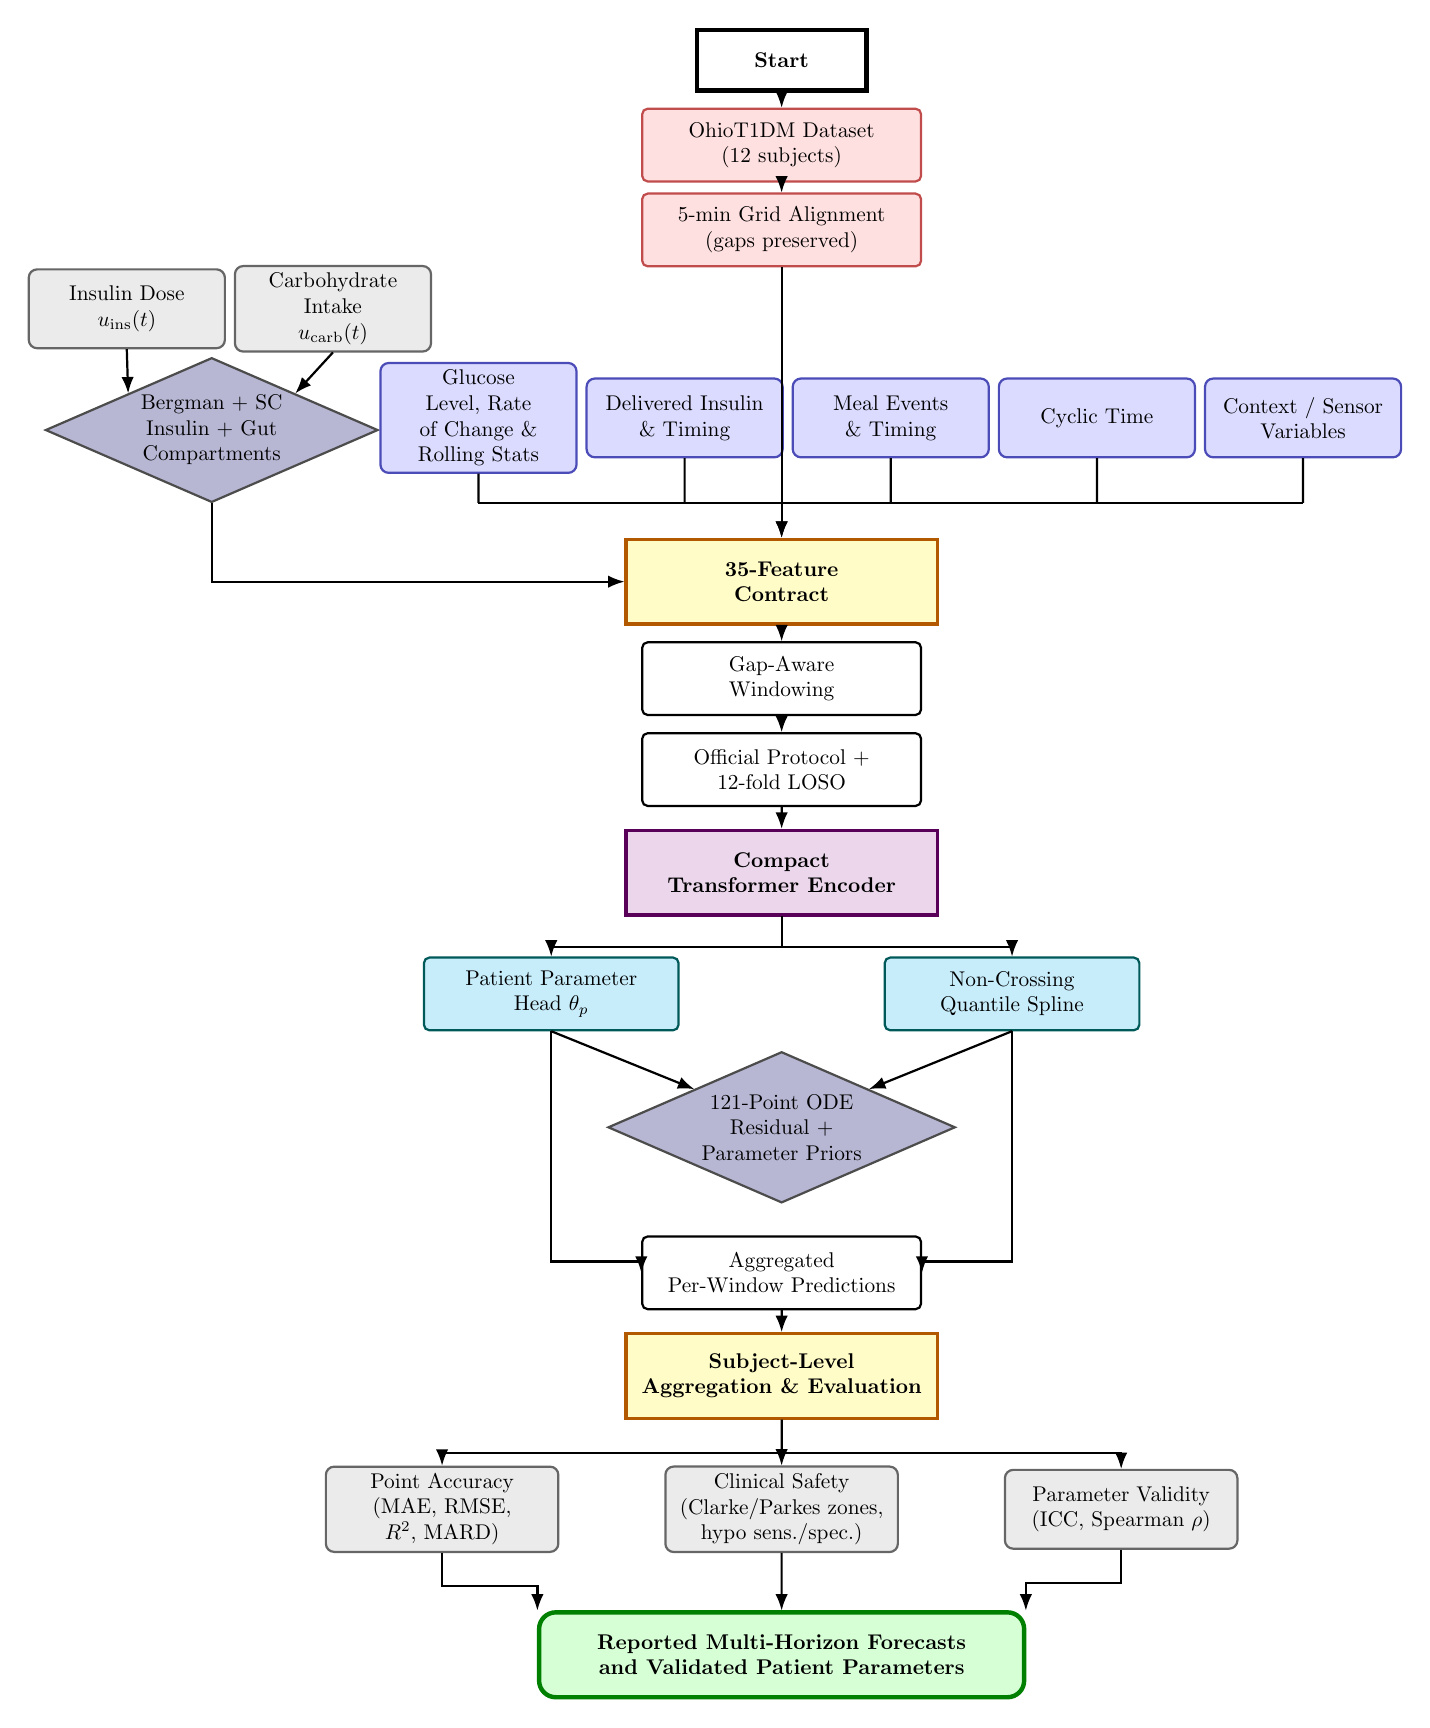
\begin{tikzpicture}[
  scale=0.77,
  transform shape,
  font=\normalsize,
  every node/.style={font=\normalsize},
  start/.style={
    rectangle, draw=black, line width=1.6pt, fill=white,
    minimum width=2.8cm, minimum height=1.0cm, align=center,
    font=\normalsize\bfseries
  },
  intake/.style={
    rectangle, rounded corners=2pt, draw=red!65!black!70, thick, fill=red!12,
    minimum width=4.6cm, minimum height=1.2cm,
    align=center, text width=4.3cm
  },
  proc/.style={
    rectangle, rounded corners=2pt, draw=black, thick, fill=white,
    minimum width=4.6cm, minimum height=1.2cm,
    align=center, text width=4.3cm
  },
  input/.style={
    rectangle, rounded corners=3pt, draw=black!60, thick, fill=black!8,
    minimum width=3.2cm, minimum height=1.3cm,
    align=center, text width=3.0cm
  },
  feat/.style={
    rectangle, rounded corners=3pt, draw=blue!60!black!70, thick, fill=blue!14,
    minimum width=3.2cm, minimum height=1.3cm,
    align=center, text width=3.0cm
  },
  hub/.style={
    chamfered rectangle,
    chamfered rectangle corners=north east and south west,
    draw=orange!70!black, very thick, fill=yellow!22,
    minimum width=5.0cm, minimum height=1.4cm,
    align=center, text width=4.7cm,
    font=\normalsize\bfseries
  },
  model/.style={
    chamfered rectangle,
    chamfered rectangle corners=north east and south west,
    draw=violet!70!black, very thick, fill=violet!16,
    minimum width=5.0cm, minimum height=1.4cm,
    align=center, text width=4.7cm,
    font=\normalsize\bfseries
  },
  head/.style={
    rectangle, rounded corners=2pt, draw=teal!70!black, thick, fill=cyan!22,
    minimum width=4.2cm, minimum height=1.2cm,
    align=center, text width=3.9cm
  },
  leaf/.style={
    rectangle, rounded corners=3pt, draw=black!60, thick, fill=black!8,
    minimum width=3.8cm, minimum height=1.3cm,
    align=center, text width=3.6cm
  },
  junction/.style={
    diamond, draw=black!70, thick, fill=blue!25!gray!45,
    aspect=2.3, align=center, inner sep=1pt,
    text width=3.0cm
  },
  final/.style={
    rectangle, rounded corners=6pt, draw=green!50!black, line width=1.6pt,
    fill=green!16,
    minimum width=8.0cm, minimum height=1.4cm,
    align=center, text width=7.6cm,
    font=\normalsize\bfseries
  },
  arr/.style={
    -{Latex[length=2.1mm]}, thick
  }
]

% Main spine
\node[start] (start) at (0,0) {Start};

\node[intake] (dataset) at (0,-1.4)
{OhioT1DM Dataset\\(12 subjects)};

\node[intake] (grid) at (0,-2.8)
{5-min Grid Alignment\\(gaps preserved)};

% Feature groups
\node[junction, text width=2.6cm] (bergman) at (-9.4,-6.1)
{Bergman + SC\\Insulin + Gut\\Compartments};

\node[feat] (fg1) at (-5.0,-5.9)
{Glucose Level, Rate\\of Change \& Rolling Stats};

\node[feat] (fg2) at (-1.6,-5.9)
{Delivered Insulin\\\& Timing};

\node[feat] (fg3) at (1.8,-5.9)
{Meal Events\\\& Timing};

\node[feat] (fg4) at (5.2,-5.9)
{Cyclic Time};

\node[feat] (fg5) at (8.6,-5.9)
{Context / Sensor\\Variables};

\node[input] (uins) at (-10.8,-4.1)
{Insulin Dose\\$u_{\text{ins}}(t)$};

\node[input] (ucarb) at (-7.4,-4.1)
{Carbohydrate Intake\\$u_{\text{carb}}(t)$};

\node[hub] (feat) at (0,-8.6)
{35-Feature\\Contract};

\node[proc] (window) at (0,-10.2)
{Gap-Aware\\Windowing};

\node[proc] (proto) at (0,-11.7)
{Official Protocol +\\12-fold LOSO};

\node[model] (xfmr) at (0,-13.4)
{Compact\\Transformer Encoder};

\node[head] (thetap) at (-3.8,-15.4)
{Patient Parameter\\Head $\theta_p$};

\node[head] (spline) at (3.8,-15.4)
{Non-Crossing\\Quantile Spline};

\node[junction] (phys) at (0,-17.6)
{121-Point ODE\\Residual +\\Parameter Priors};

\node[proc] (agg) at (0,-20.0)
{Aggregated\\Per-Window Predictions};

\node[hub] (eval) at (0,-21.7)
{Subject-Level\\Aggregation \& Evaluation};

\node[leaf] (acc) at (-5.6,-23.9)
{Point Accuracy\\(MAE, RMSE, $R^2$, MARD)};

\node[leaf] (safe) at (0,-23.9)
{Clinical Safety\\(Clarke/Parkes zones,\\hypo sens./spec.)};

\node[leaf] (valid) at (5.6,-23.9)
{Parameter Validity\\(ICC, Spearman $\rho$)};

\node[final] (outcome) at (0,-26.3)
{Reported Multi-Horizon Forecasts\\and Validated Patient Parameters};

% Mechanistic branch
\draw[arr] (uins.south) -- (bergman.north west);
\draw[arr] (ucarb.south) -- (bergman.north east);
\draw[arr] (bergman.south) |- (feat.west);

% Feature merge
\draw[thick] (fg1.south) -- (-5.0,-7.3);
\draw[thick] (fg2.south) -- (-1.6,-7.3);
\draw[thick] (fg3.south) -- (1.8,-7.3);
\draw[thick] (fg4.south) -- (5.2,-7.3);
\draw[thick] (fg5.south) -- (8.6,-7.3);
\draw[thick] (-5.0,-7.3) -- (8.6,-7.3);
\draw[arr] (0,-7.3) -- (feat.north);

% Main vertical spine
\draw[arr] (start) -- (dataset);
\draw[arr] (dataset) -- (grid);
\draw[arr] (grid.south) -- (feat.north);
\draw[arr] (feat) -- (window);
\draw[arr] (window) -- (proto);
\draw[arr] (proto) -- (xfmr);

% Transformer heads
\draw[arr] (xfmr.south) -- ++(0,-0.5) -| (thetap.north);
\draw[arr] (xfmr.south) -- ++(0,-0.5) -| (spline.north);

% Physics check
\draw[arr] (thetap.south) -- (phys.north west);
\draw[arr] (spline.south) -- (phys.north east);

% Forward path
\draw[arr] (thetap.south) -- ++(0,-3.8) -| (agg.west);
\draw[arr] (spline.south) -- ++(0,-3.8) -| (agg.east);

\draw[arr] (agg) -- (eval);

% Evaluation
\draw[arr] (eval.south) -- ++(0,-0.55) -| (acc.north);
\draw[arr] (eval) -- (safe);
\draw[arr] (eval.south) -- ++(0,-0.55) -| (valid.north);

% Final outcome
\draw[arr] (acc.south) -- ++(0,-0.55) -| (outcome.north west);
\draw[arr] (safe) -- (outcome);
\draw[arr] (valid.south) -- ++(0,-0.55) -| (outcome.north east);

\end{tikzpicture}

\caption{\small\textit{Audited digital-twin pipeline. OhioT1DM glucose and related patient data are aligned to five-minute intervals and processed through two parallel paths: a deep-learning model and a physiological model. The deep-learning model predicts future glucose levels and estimates patient-specific parameters, while the physiological model represents insulin and glucose dynamics. Physiological information is used both as an input to the model and as a training constraint to improve prediction consistency.
}}
\label{fig:pipeline}
\end{figure*}

\subsection{Mechanistic Patient Model}

The physiological core extends the Bergman minimal model and its insulin-sensitivity index~\cite{ref1,ref32} as shown in \ (Eqs.~\eqref{eq:2}-\eqref{eq:4}):
\begin{align}
\dot{G} &= -(p_1 + X)\,G + p_1 G_b + \frac{R_a(t)}{V_G}, \label{eq:2}\\
\dot{X} &= -p_2 X + p_3 (I - I_b), \label{eq:3}\\
\dot{I} &= -nI + \frac{1000}{V_I}\cdot\frac{S_2}{t_{\max,I}}. \label{eq:4}
\end{align}

Here $G$ is glucose, $I$ plasma insulin, $X$ remote insulin action, and subscript $b$ denotes basal state. All rates are per minute. Basal subtraction in (\ref{eq:3}) is essential: at $I = I_b$, $X^* = 0$ and $G = G_b$ is an equilibrium. Driving the equation with total insulin instead would create a spurious downward glucose attractor.

The patient-specific insulin sensitivity is the steady-state gain as shown in \ (Eq.~\eqref{eq:5}):
\begin{equation}
S_I = \frac{p_3}{p_2}, \qquad X_{ss} = S_I (I - I_b),
\label{eq:5}
\end{equation}
with units mL\,$\mu$U$^{-1}$min$^{-1}$. Parameters are mapped by sigmoid functions into physiologically sourced intervals informed by minimal-model studies in insulin-dependent diabetes~\cite{ref33} and regularized toward population anchors. Consequently, plausible range alone is not evidence of identifiability; external and stability checks are required.

Subcutaneous insulin absorption follows a two-compartment model~\cite{ref34} as shown in (\ Eqs.~\eqref{eq:6}-\eqref{eq:8}):
\begin{align}
\dot{S}_1 &= u_{\text{ins}}(t) - \frac{S_1}{t_{\max,I}}, \label{eq:6}\\
\dot{S}_2 &= \frac{S_1}{t_{\max,I}} - \frac{S_2}{t_{\max,I}}. \label{eq:7}
\end{align}

For an impulse dose $D$, insulin on board is
\begin{equation}
S_1 + S_2 = D\,e^{-t/t_{\max,I}}\left(1 + \frac{t}{t_{\max,I}}\right),
\label{eq:8}
\end{equation}
which starts at $D$ and decreases monotonically. Carbohydrate absorption follows compartmental meal models used in T1D simulation~[\hyperref[ref35label]{35}-\hyperref[ref37label]{37}] and is represented by stomach and gut states,as shown in (\ Eqs.\eqref{eq:9}-\eqref{eq:11}):
\begin{align}
\dot{Q}_{\text{sto}} &= -k_{\text{gri}} Q_{\text{sto}} + u_{\text{carb}}(t), \label{eq:9}\\
\dot{Q}_{\text{gut}} &= k_{\text{gri}} Q_{\text{sto}} - k_{\text{abs}} Q_{\text{gut}}, \label{eq:10}\\
R_a(t) &= f\, k_{\text{abs}} Q_{\text{gut}}(t), \label{eq:11}
\end{align}
so carbohydrate on board is $Q_{\text{sto}} + Q_{\text{gut}}$ and absorbed mass is conserved. For implementation, the non-glucose compartments are collected as shown in (\ Eq.\eqref{eq:12}):
\begin{equation}
\mathbf{z} = {[S_1, S_2, I, Q_{\text{sto}}, Q_{\text{gut}}, X]}^{\mathsf T}, \quad \mathbf{u} = {[u_{\text{ins}}, u_{\text{carb}}, I_b]}^{\mathsf T}.
\label{eq:12}
\end{equation}

With parameters held constant over one grid interval, $\dot{\mathbf{z}} = A\mathbf{z} + B\mathbf{u}$ has the exact zero-order-hold update (a standard control-theory discretization technique, not attributed to a specific glucose-modeling source) as shown in (\ Eq.\eqref{eq:13}):
\begin{equation}
\mathbf{z}_{k+1} = A_d \mathbf{z}_k + B_d \mathbf{u}_k, \qquad
\begin{bmatrix} A_d & B_d \\ 0 & I \end{bmatrix} = \exp\!\left(\Delta \begin{bmatrix} A & B \\ 0 & 0 \end{bmatrix}\right).
\label{eq:13}
\end{equation}

This matrix-exponential formulation preserves the affine basal term through the explicit $I_b$ input and avoids the accumulated integration error of a coarse explicit solver.

\subsection{Feature Contract and Forecasting Network}

Each timestep contains 35 named features in six groups: glucose level, multiscale rates of change and rolling statistics; delivered insulin and timing; meals and timing; mechanistic states (IOB, COB, plasma insulin, remote action, and glucose appearance); cyclic time; and context/sensor variables. A two-hour window $X \in \mathbb{R}^{24 \times 35}$ is standardized using training-only statistics.

The forecasting network is deliberately small (approximately 79,000 parameters) because the effective sample size is limited. A linear projection and positional encoding feed a Transformer encoder~\cite{ref38}. As per (\ Eq.\eqref{eq:14})Attention pooling gives :
\begin{equation}
z = \sum_{t=1}^{24} \alpha_t h_t, \qquad \alpha_t = \frac{\exp(w^\top h_t)}{\sum_j \exp(w^\top h_j)},
\label{eq:14}
\end{equation}
avoiding the equal weighting of old and recent measurements induced by mean pooling.

One head estimates the ten-component subject parameter vector $\theta_p$. A second predicts a cubic B-spline trajectory as shown in (\ Eq.\eqref{eq:15}) :
\begin{equation}
G_\theta(t) = G_0 + \sum_{k=1}^{K} c_k \big(B_k(t) - B_k(0)\big),
\label{eq:15}
\end{equation}
which anchors every trajectory at the last observed glucose $G_0$. Median knot values are unconstrained, whereas lower and upper quantiles are generated by positive softplus offsets in glucose units; quantiles therefore cannot cross. A learned trust gate $g = \sigma(\gamma)$ controls the contribution of the mechanistic prior, with $g \approx 0.10$ at initialization. Predictions at all four horizons are evaluated from the spline.

\subsection{Training Objective}

The data objective combines Huber's robust loss~\cite{ref39} for the median with the pinball loss used in quantile regression~\cite{ref40} for lower and upper quantiles as shown in (\ Eq.\eqref{eq:16}):
\begin{equation}
\mathcal{L}_{\text{data}} = \mathcal{L}_{\text{Huber}}(y, \hat{y}_{0.5}) + \sum_{q \in \{0.1, 0.9\}} \rho_q(y - \hat{y}_q),
\label{eq:16}
\end{equation}
where $\rho_q(u) = u(q - \mathbb{1}_{u<0})$. Physics residuals are evaluated at 121 collocation points over the two-hour forecast and normalized by physiological scales, following the residual-minimization principle of PINNs~\cite{ref8}. The full objective is shown in (\ Eq.\eqref{eq:17}):
\begin{equation}
\mathcal{L} = \mathcal{L}_{\text{data}} + \lambda_{\text{phys}} \mathcal{L}_{\text{phys}} + \lambda_{\text{prior}} \mathcal{L}_{\text{prior}} + \lambda_{\text{stab}} \mathcal{L}_{\text{within-subject}}.
\label{eq:17}
\end{equation}

Closed-form state updates replace a memory-intensive differentiable ODE solver. Adaptive loss weighting was motivated by work on gradient imbalance and uncertainty-based multi-objective learning~[\hyperref[ref41label]{41}-\hyperref[ref42label]{42}]. The selected A7 configuration applies physics from epoch one; a data-first curriculum was rejected because validation optima repeatedly occurred before the curriculum became selectable.

\subsection{Evaluation and Statistical Analysis}

The official temporal protocol uses each subject's earlier data for training. LOSO trains on 11 subjects and evaluates the held-out subject on the identical test windows. Metrics are computed per subject and summarized as mean $\pm$ SD\@. Persistence predicts $\hat{G}(t+h) = G(t)$. Skill is $1 - \text{RMSE}_{\text{model}}/\text{RMSE}_{\text{persistence}}$, computed from the cohort-mean RMSEs.

Clinical evaluation includes Clarke and Parkes zones~[\hyperref[ref43label]{43}-\hyperref[ref45label]{45}], consensus CGM ranges~\cite{ref52}, coefficient-of-variation ratio, and Kovatchev low/high blood-glucose risk indices~[\hyperref[ref46label]{46}-\hyperref[ref47label]{47}], together with hypoglycemia sensitivity, specificity, precision, and quantile calibration. Paired model comparisons use the Wilcoxon signed-rank test~\cite{ref48} across 12 subjects with Holm multiplicity correction~\cite{ref49}; bootstrap intervals resample subjects, never overlapping windows. Test--retest reliability of $S_I$ is measured with one-way ICC(1)~\cite{ref50}, and concurrent validity uses Spearman rank correlation~\cite{ref51}.

\subsection{Preregistered Outcomes and Falsification Criteria}

The analysis plan, primary/secondary endpoints, and falsification thresholds were formally committed prior to inspecting test outcomes, following rigorous open-science preregistration practice~\cite{ref79}. Specifically, the complete protocol and falsification criteria were committed to the public version-controlled repository (\url{https://github.com/sammyyakk/digital-twin}) under timestamped git commit \texttt{3baf636fce11ed5780d3e79aeee6ed8b4a5e02d4} (dated Sat Jul 25 17:49:43 2026 +0530, \texttt{docs/PREREGISTRATION.md}) before test-set evaluation began.

The primary outcome is 30-minute MAE under the official protocol for the physiology-focused branch. Secondary outcomes include all horizons under both protocols, persistence skill, Clarke, Parkes, and PRED-EGA distributions, the ablation matrix, quantile calibration, and the three $S_I$ validation checks. Table~\ref{tab:falsification} records the criteria that were fixed in advance; unmet criteria are reported as failures rather than redefined after inspection.

No asymmetric hypoglycemia/hyperglycemia point-loss term is permitted, because such a term would directly optimize the safety table later used as evidence. The test set is evaluated only after model selection, and the official protocol is never described as subject-disjoint generalization.

\subsection{Reproducibility, Hardware, and Latency}

All models were implemented in PyTorch 2.10 (CUDA 12.8) and trained using AdamW with learning rate $\eta = 5 \times 10^{-4}$, weight decay $0.03$, batch size $256$, and gradient clipping at maximum $L_2$ norm $1.0$. Training proceeded for at most 70 epochs with early stopping triggered after 12 epochs without improvement in validation mean MAE across horizons. The hyperparameter search space covered encoder depth $\in \{2, 4\}$ layers, hidden dimension $d_{\text{model}} \in \{64, 128\}$, attention heads $\in \{4, 8\}$, feed-forward dimension $d_{\text{ff}} \in \{128, 512\}$, dropout $\in \{0.1, 0.2\}$, pooling mode $\in \{\text{attention}, \text{mean}, \text{last}\}$, and physics loss weighting (fixed $\lambda_{\text{phys}} \in [0.01, 1.0]$ vs.\ Kendall homoscedastic uncertainty weighting).

Experiments were run on a single machine equipped with an NVIDIA GeForce RTX 2050 Laptop GPU (4~GB GDDR6 VRAM), an Intel Core host processor, and Linux. Training required approximately $23$ seconds per epoch ($\sim 4.5$ minutes total to convergence per run). Runtime inference latency per single forecast window (batch size $1$) was empirically measured across 100 consecutive forward passes: $15.25 \pm 4.07$~ms on GPU (median $13.21$~ms, 95th percentile $25.07$~ms) and $6.33 \pm 0.18$~ms on CPU (median $6.31$~ms), easily satisfying real-time deployment constraints for a 5-minute CGM sampling interval. Complete code, data-processing pipelines, and configs are available at \url{https://github.com/sammyyakk/digital-twin}.

Integrated gradients (IG)~\cite{ref54} uses the standardized training mean as its zero baseline as shown in (\ Eq.\eqref{eq:18}):
\begin{equation}
\text{IG}_i(x) = (x_i - x_i') \int_0^1 \frac{\partial f(x' + \alpha(x - x'))}{\partial x_i}\, d\alpha.
\label{eq:18}
\end{equation}

Because IG shows an unresolved completeness violation, every interpretation is cross-checked with model-agnostic permutation importance, following the perturbation principle popularized for random forests~\cite{ref55}.

\begin{table*}[t]
\centering
\caption{Preregistered success and falsification criteria}
\label{tab:falsification}
\footnotesize
\begin{tabular}{>{\raggedright\arraybackslash}p{2.6cm}>{\raggedright\arraybackslash}p{5.6cm}>{\raggedright\arraybackslash}p{5.8cm}>{\raggedright\arraybackslash}p{2.4cm}}
\toprule
Claim & Criterion fixed before test evaluation & Interpretation & Ref. \\
\midrule
Beats persistence & 30-minute MAE below persistence in at least 10 of 12 subjects & Requires broadly distributed improvement, not a pooled gain driven by a few subjects. & [\hyperref[ref30label]{30}-\hyperref[ref31label]{31}],~\cite{ref57} \\
Field-competitive point accuracy & 30-minute MAE $\leq$ 13.5 mg/dL & A field-relative target, explicitly not a clinical acceptability threshold. &~\cite{ref31},~[\hyperref[ref43label]{43}-\hyperref[ref44label]{44}],~\cite{ref64} \\
Physics improves accuracy & Physics arm beats A0 at 30 minutes and survives paired Wilcoxon testing with Holm correction & If unmet, physics is not credited with point-accuracy improvement. & [\hyperref[ref48label]{48}-\hyperref[ref49label]{49}] \\
$S_I$ is subject-specific & Between-subject CV $>$ 10\% & Rejects a parameter head collapsed to one population value. &~\cite{ref1,ref32} \\
$S_I$ is stable & ICC(1) $>$ 0.5 on disjoint within-subject blocks & Rejects a window-level nuisance variable that merely absorbs prediction error. &~\cite{ref50,ref76} \\
$S_I$ is externally consistent & Spearman $\rho < 0$ versus total daily dose, with a subject-bootstrap 95\% CI excluding zero & Evaluated separately under personalized and LOSO protocols. &~\cite{ref51},~[\hyperref[ref77label]{77}-\hyperref[ref78label]{78}] \\
\bottomrule
\end{tabular}
\end{table*}


%=================================================================
\section{Results}

\subsection{Baseline Validation and Data Accounting}

Persistence RMSE on the 2018 cohort is $22.52 \pm 2.56$~mg/dL at 30 minutes and $36.19 \pm 3.26$~mg/dL at 60 minutes, within $0.02$~mg/dL of both independently published no-change baselines at 30 minutes and within $0.41$~mg/dL of the published 60-minute value[\hyperref[ref56label]{56}-\hyperref[ref57label]{57}]. This close agreement validates the complete evaluation pipeline, including data parsing, five-minute grid alignment, horizon construction, persistence-target generation, RMSE computation, and subject-level aggregation Table~\ref{tab:windows}. The retained-window accounting further confirms that the reported metrics are computed on the intended 26,498 common test windows. 

\begin{table}[t]
\centering
\caption{Window accounting after integrity filtering}
\label{tab:windows}
\footnotesize
\begin{tabular}{lr}
\toprule
Quantity & Value \\
\midrule
Subjects / CGM observations & 12 / 166,443 \\
Candidate windows & 187,780 \\
Retained windows & 141,100 (75.1\%) \\
Incomplete input span & 36,395 \\
Missing real target & 10,285 \\
Common test windows & 26,498 \\
Effective independent windows & $\approx 2{,}800$ \\
\bottomrule
\end{tabular}
\end{table}

\subsection{Official-Protocol Forecast Accuracy}

Table~\ref{tab:official} and Fig.~\ref{fig:summary} show that the model improves on persistence at every horizon. All 12 subjects improve at 30 minutes; subject-level MAE skill ranges from 12.2\% to 31.6\%. The decline in $R^2$ with horizon is expected because future meals, boluses, and activity are absent from the input.

\pgfplotstableread[col sep=comma]{data/mae_by_horizon.csv}\maetable
\pgfplotstableread[col sep=comma]{data/rmse_by_horizon.csv}\rmsetable
\pgfplotstablegetelem{0}{mean}\of\maetable \global\let\maePersA=\pgfplotsretval
\pgfplotstablegetelem{1}{mean}\of\maetable \global\let\maePersB=\pgfplotsretval
\pgfplotstablegetelem{2}{mean}\of\maetable \global\let\maePersC=\pgfplotsretval
\pgfplotstablegetelem{3}{mean}\of\maetable \global\let\maePersD=\pgfplotsretval
\pgfplotstablegetelem{4}{mean}\of\maetable \global\let\maeModA=\pgfplotsretval
\pgfplotstablegetelem{5}{mean}\of\maetable \global\let\maeModB=\pgfplotsretval
\pgfplotstablegetelem{6}{mean}\of\maetable \global\let\maeModC=\pgfplotsretval
\pgfplotstablegetelem{7}{mean}\of\maetable \global\let\maeModD=\pgfplotsretval
\pgfplotstablegetelem{0}{mean}\of\rmsetable \global\let\rmsePersA=\pgfplotsretval
\pgfplotstablegetelem{1}{mean}\of\rmsetable \global\let\rmsePersB=\pgfplotsretval
\pgfplotstablegetelem{2}{mean}\of\rmsetable \global\let\rmsePersC=\pgfplotsretval
\pgfplotstablegetelem{3}{mean}\of\rmsetable \global\let\rmsePersD=\pgfplotsretval
\pgfplotstablegetelem{4}{mean}\of\rmsetable \global\let\rmseModA=\pgfplotsretval
\pgfplotstablegetelem{5}{mean}\of\rmsetable \global\let\rmseModB=\pgfplotsretval
\pgfplotstablegetelem{6}{mean}\of\rmsetable \global\let\rmseModC=\pgfplotsretval
\pgfplotstablegetelem{7}{mean}\of\rmsetable \global\let\rmseModD=\pgfplotsretval
\pgfmathsetmacro{\skillA}{100*(1-\rmseModA/\rmsePersA)}
\pgfmathsetmacro{\skillB}{100*(1-\rmseModB/\rmsePersB)}
\pgfmathsetmacro{\skillC}{100*(1-\rmseModC/\rmsePersC)}
\pgfmathsetmacro{\skillD}{100*(1-\rmseModD/\rmsePersD)}


% Core packages


% Paragraphs
\begin{figure*}[t]
\centering

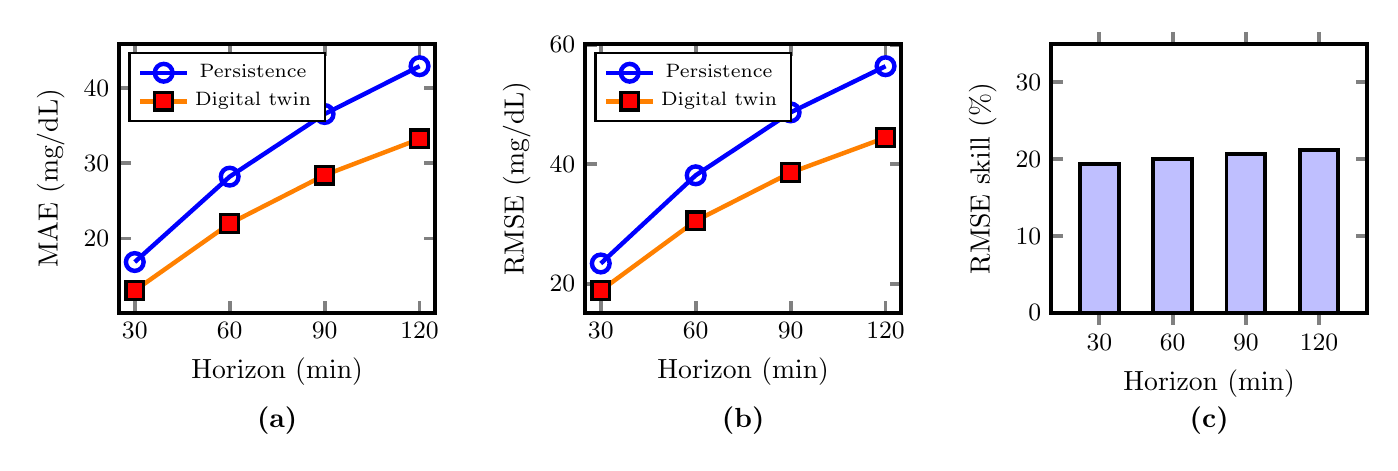
\begin{tikzpicture}
\begin{groupplot}[
  group style={group size=3 by 1, horizontal sep=1.9cm},
  width=5.6cm, height=5.0cm,
  xlabel={Horizon (min)},
  xtick={30,60,90,120},
  axis line style={line width=1.4pt},
  tick style={line width=1.4pt},
  label style={font=\normalsize},
  tick label style={font=\small},
  title style={font=\normalsize\bfseries, yshift=-0.7em},
]

% ---------- (a) MAE ----------
\nextgroupplot[
  ylabel={MAE (mg/dL)},
  xmin=25, xmax=125,
  legend pos=north west,
  legend style={
    font=\scriptsize,
    line width=0.8pt,
    draw=black,
    inner xsep=3pt,
    inner ysep=2pt
},
  title={(a)},
  title style={at={(0.5,-0.30)}, anchor=north},
]
\addplot[
  color=blue, line width=1.6pt, mark=o, mark options={scale=1.6, line width=1.6pt, fill=none},
] coordinates {
  (30,16.87) (60,28.22) (90,36.55) (120,42.90)
};
\addlegendentry{Persistence}

\addplot[
  color=orange, line width=1.6pt, mark=square*,
  mark options={scale=1.6, line width=1.2pt, fill=red, draw=black},
] coordinates {
  (30,13.08) (60,21.98) (90,28.42) (120,33.23)
};
\addlegendentry{Digital twin}

% ---------- (b) RMSE ----------
\nextgroupplot[
  ylabel={RMSE (mg/dL)},
  xmin=25, xmax=125,
  legend pos=north west,
  legend style={
    font=\scriptsize,
    line width=0.8pt,
    draw=black,
    inner xsep=3pt,
    inner ysep=2pt
},
  title={(b)},
  title style={at={(0.5,-0.30)}, anchor=north},
]
\addplot[
  color=blue, line width=1.6pt, mark=o, mark options={scale=1.6, line width=1.6pt, fill=none},
] coordinates {
  (30,23.37) (60,38.15) (90,48.69) (120,56.43)
};
\addlegendentry{Persistence}

\addplot[
  color=orange, line width=1.6pt, mark=square*,
  mark options={scale=1.6, line width=1.2pt, fill=red, draw=black},
] coordinates {
  (30,18.84) (60,30.52) (90,38.60) (120,44.46)
};
\addlegendentry{Digital twin}

% ---------- (c) RMSE skill ----------
\nextgroupplot[
  ylabel={RMSE skill (\%)},
  ybar,
  bar width=14pt,
  ymin=0, ymax=35,
  xtick=data,
  symbolic x coords={30,60,90,120},
  enlarge x limits=0.22,
  title={(c)},
  title style={at={(0.5,-0.30)}, anchor=north},
]
\addplot[
  fill=blue!25, draw=black, line width=1.4pt,
] coordinates {
  (30,19.4) (60,20.0) (90,20.7) (120,21.2)
};
\end{groupplot}
\end{tikzpicture}

\caption{\small\textit{Official-protocol accuracy summary at 30/60/90/120 minutes. 2a and 2b: MAE and RMSE for persistence versus the digital twin both rise with horizon, but the gap between the two curves widens rather than closes, showing the model's advantage over naive persistence is not a short-horizon artifact. 2c: the resulting RMSE skill stays essentially flat at 19--21\% across all four horizons.}}
\label{fig:summary}
\end{figure*}





\begin{table*}[t]
\centering
\caption{Official personalized protocol: mean $\pm$ SD across subjects (($\mathrm{mg/dL}$) unless noted)}
\label{tab:official}
\footnotesize
\begin{tabular}{lrrrrrrr}
\toprule
Horizon & Persistence MAE & Model MAE & Persistence RMSE & Model RMSE & RMSE skill & $R^2$ & MARD \\
\midrule
30 min & 16.87 $\pm$ 1.92 & \textbf{13.08 $\pm$ 1.73} & 23.37 & \textbf{18.84 $\pm$ 2.58} & 19.4\% & 0.885 & 8.79\% \\
60 min & 28.22 $\pm$ 3.24 & \textbf{21.98 $\pm$ 2.96} & 38.15 & \textbf{30.52 $\pm$ 3.98} & 20.0\% & 0.700 & 14.76\% \\
90 min & 36.55 $\pm$ 4.00 & \textbf{28.42 $\pm$ 3.89} & 48.69 & \textbf{38.60 $\pm$ 5.05} & 20.7\% & 0.523 & 19.14\% \\
120 min & 42.90 $\pm$ 4.46 & \textbf{33.23 $\pm$ 4.45} & 56.43 & \textbf{44.46 $\pm$ 5.62} & 21.2\% & 0.368 & 22.37\% \\
\bottomrule
\end{tabular}
\end{table*}

\subsection{Cross-Subject Generalization}

At 30 minutes, LOSO remains better than persistence in all 12 subjects by MAE (10 of 12 by RMSE), but is consistently worse than the personalized protocol. As Fig.~\ref{fig:matched_protocol_comparison} shows, the personalization gap grows with horizon, consistent with increasing dependence on individual insulin kinetics and routine.

\pgfplotstableread[col sep=comma]{data/loso_leaderboard_mae.csv}\losotable
\pgfplotstablegetelem{0}{mean}\of\maetable \global\let\persA=\pgfplotsretval
\pgfplotstablegetelem{1}{mean}\of\maetable \global\let\persB=\pgfplotsretval
\pgfplotstablegetelem{2}{mean}\of\maetable \global\let\persC=\pgfplotsretval
\pgfplotstablegetelem{3}{mean}\of\maetable \global\let\persD=\pgfplotsretval
\pgfplotstablegetelem{4}{mean}\of\maetable \global\let\persoA=\pgfplotsretval
\pgfplotstablegetelem{5}{mean}\of\maetable \global\let\persoB=\pgfplotsretval
\pgfplotstablegetelem{6}{mean}\of\maetable \global\let\persoC=\pgfplotsretval
\pgfplotstablegetelem{7}{mean}\of\maetable \global\let\persoD=\pgfplotsretval
\pgfplotstablegetelem{4}{mae_mean}\of\losotable \global\let\losoA=\pgfplotsretval
\pgfplotstablegetelem{5}{mae_mean}\of\losotable \global\let\losoB=\pgfplotsretval
\pgfplotstablegetelem{6}{mae_mean}\of\losotable \global\let\losoC=\pgfplotsretval
\pgfplotstablegetelem{7}{mae_mean}\of\losotable \global\let\losoD=\pgfplotsretval

\begin{figure}[t]
\centering

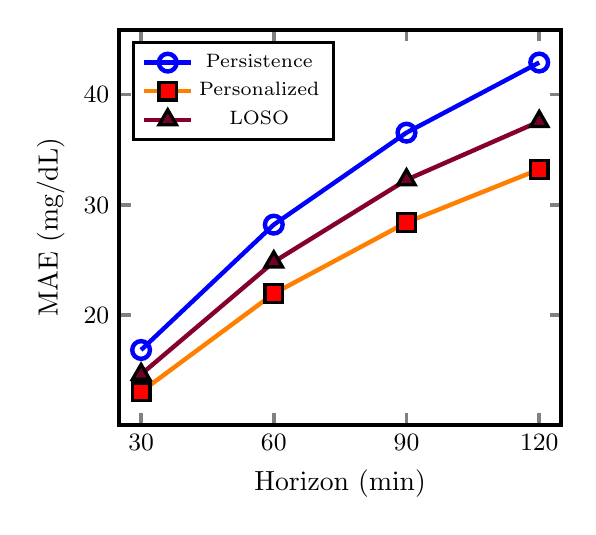
\begin{tikzpicture}
\begin{axis}[
  width= 7.2cm, height=6.6 cm,
  xlabel={Horizon (min)},
  ylabel={MAE (mg/dL)},
  xtick={30,60,90,120},
  xmin=25, xmax=125,
  axis line style={line width=1.4pt},
  tick style={line width=1.4pt},
  label style={font=\normalsize},
  tick label style={font=\small},
  legend pos=north west,
  legend style={font=\scriptsize, line width=1pt, draw=black},
]

\addplot[
  color=blue, line width=1.6pt, mark=o, mark options={scale=1.6, line width=1.6pt, fill=none},
] coordinates {
  (30,16.87) (60,28.22) (90,36.55) (120,42.90)
};
\addlegendentry{Persistence}

\addplot[
  color=orange, line width=1.6pt, mark=square*,
  mark options={scale=1.6, line width=1.2pt, fill=red, draw=black},
] coordinates {
  (30,13.08) (60,21.98) (90,28.42) (120,33.23)
};
\addlegendentry{Personalized}

\addplot[
  color=purple!70!black, line width=1.6pt, mark=triangle*,
  mark options={scale=1.8, line width=1.2pt, fill=purple!60!black, draw=black},
] coordinates {
  (30,14.66) (60,24.85) (90,32.28) (120,37.56)
};
\addlegendentry{LOSO}

\end{axis}
\end{tikzpicture}

\caption{\small\textit{Matched-protocol comparison across 30, 60, 90, and 120-minute horizons. Persistence, personalized, and LOSO models are evaluated on identical windows. LOSO keeps a roughly constant MAE advantage of about 12\% over persistence at every horizon, while its gap to the personalized model widens from 1.6 to 4.3~mg/dL, indicating a greater benefit from within-subject history for extended forecasting.}}
\label{fig:matched_protocol_comparison}
\end{figure}


\subsection{Physics Ablations}

No physics configuration significantly outperforms the no-physics A0 baseline after Holm correction (Table~\ref{tab:ablation}; Fig.~\ref{fig:ablationfig}). A7 is nominally best and improves 9 of 12 subjects, but its corrected $p = 0.105$. Per-patient parameters are accuracy-neutral: A3 and population-fixed A4 differ by 0.07–0.23 mg/dL at 30/60 min, widening to 0.76 mg/dL at 120 min. In contrast with earlier physiology-informed OhioT1DM studies that primarily reported forecast accuracy~[\hyperref[ref58label]{58}-\hyperref[ref59label]{59}], this ablation separates parameter estimation from predictive gain. The defensible value of physics is not superior point accuracy; it is access to a stable physiological parameter and informative mechanistic states without a material accuracy penalty.

\textit{Status of Arms A5 and A6:} The ablation protocol initially designed arms A0 through A7, but arms A5 and A6 were dropped for verified technical reasons rather than omitted post hoc:
\begin{itemize}
    \item \textbf{Ablation A5 (Simulation pretraining):} Intended to evaluate transfer learning from UVA/Padova simulator traces. A pipeline audit discovered a defect in the legacy meal generator: meal times were re-sampled inside the inner per-step integration loop, resulting in an unphysiological average of $\sim 0.6$ meals per day rather than $3$ meals per day. Because this corrupted the synthetic postprandial training distribution, A5 was formally blocked to avoid training on invalid synthetic data.
    \item \textbf{Ablation A6 (Legacy hand-rolled kernels):} Formulated to quantify the benefit of deriving IOB/COB from the mass-conserving Bergman ODE versus legacy heuristic kernels (which featured an unnormalized exponential carbohydrate decay and a time-reversed insulin action curve). Rather than maintaining a defective heuristic pipeline, the value of the principled compartmental states is quantified directly via feature attribution (Section~\ref{sec:attribution}), where they carry $27.1\%$ of total model attribution.
\end{itemize}


\begin{table*}[t]
\centering

\caption{Ablation matrix. mae at all horizons; clarke a and hypoglycemia metrics at 30 min. hypo bias is mean error for glucose below 70 ($\mathrm{mg/dL}$)}
\label{tab:ablation}
\footnotesize
\setlength{\tabcolsep}{4.5pt}
\begin{tabular}{llrrrrrrrl}
\toprule
Arm & Configuration & MAE30 & MAE60 & MAE90 & MAE120 & Clarke A & Hypo sens. & Hypo bias & Gives $S_I$ \\
\midrule
A0 & Transformer, no physics & 13.51 & 22.82 & 29.74 & 34.93 & 89.4\% & 0.637 & +7.29 & no \\
A1 & Penalty PINN, fixed $\lambda=0.1$ & 13.68 & 23.47 & 30.93 & 36.22 & 88.9\% & 0.502 & +11.29 & no \\
A2 & Adaptive penalty, per patient & 13.58 & 23.35 & 30.59 & 35.74 & 89.0\% & 0.499 & +11.03 & yes \\
A3 & Hybrid prior, curriculum & 13.65 & 23.12 & 30.02 & 34.83 & 89.0\% & 0.485 & +10.95 & yes \\
A4 & Hybrid, fixed population parameters & 13.58 & 23.35 & 30.57 & 35.59 & 89.1\% & 0.517 & +10.18 & no \\
A7 & Hybrid, full physics from epoch 1 & \textbf{13.25} & \textbf{22.29} & \textbf{28.77} & \textbf{33.38} & \textbf{89.8\%} & 0.608 & +8.61 & yes \\
\bottomrule
\end{tabular}
\end{table*}

\pgfplotstableread[col sep=comma]{data/leaderboard_mae_A0.csv}\tabA
\pgfplotstableread[col sep=comma]{data/leaderboard_mae_A1.csv}\tabB
\pgfplotstableread[col sep=comma]{data/leaderboard_mae_A2.csv}\tabC
\pgfplotstableread[col sep=comma]{data/leaderboard_mae_A3.csv}\tabD
\pgfplotstableread[col sep=comma]{data/leaderboard_mae_A4.csv}\tabE
\pgfplotstableread[col sep=comma]{data/leaderboard_mae_A7.csv}\tabF
\pgfplotstablegetelem{4}{mae_mean}\of\tabA \global\let\ablA=\pgfplotsretval
\pgfplotstablegetelem{4}{mae_mean}\of\tabB \global\let\ablB=\pgfplotsretval
\pgfplotstablegetelem{4}{mae_mean}\of\tabC \global\let\ablC=\pgfplotsretval
\pgfplotstablegetelem{4}{mae_mean}\of\tabD \global\let\ablD=\pgfplotsretval
\pgfplotstablegetelem{4}{mae_mean}\of\tabE \global\let\ablE=\pgfplotsretval
\pgfplotstablegetelem{4}{mae_mean}\of\tabF \global\let\ablF=\pgfplotsretval

\begin{figure}[t]
\centering
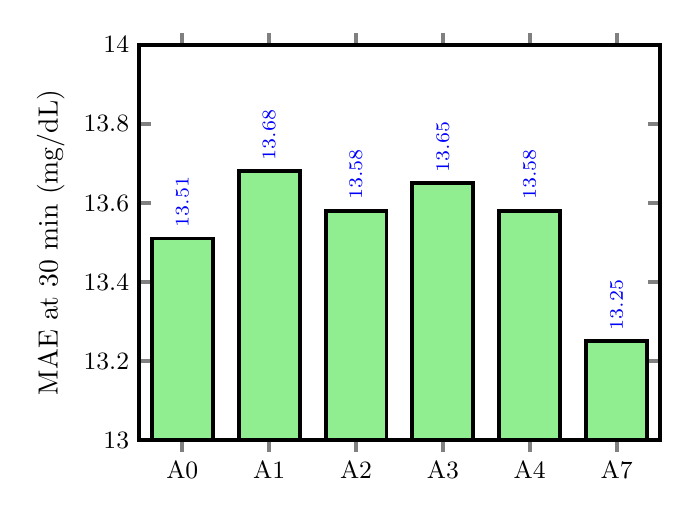
\begin{tikzpicture}
\begin{axis}[
  width=8.2cm, height=6.6cm,
  ybar,
  bar width=22pt,
  xlabel={},
  ylabel={MAE at 30 min (mg/dL)},
  symbolic x coords={A0,A1,A2,A3,A4,A7},
  xtick=data,
  ymin=13, ymax=14,
  axis line style={line width=1.4pt},
  tick style={line width=1.4pt},
  label style={font=\normalsize},
  tick label style={font=\small},
  nodes near coords,
  nodes near coords style={font=\scriptsize, color=blue, rotate=90, anchor=west},
  every node near coord/.append style={/pgf/number format/.cd, fixed, precision=2},
]

\addplot[
  fill={rgb,255:red,144;green,238;blue,144}, draw=black, line width=1.4pt,
] coordinates {
  (A0,13.51) (A1,13.68) (A2,13.58) (A3,13.65) (A4,13.58) (A7,13.25)
};

\end{axis}

\end{tikzpicture}
\caption{\small\textit{Point-accuracy ablation at 30 minutes comparing six physics configurations (A0-A4,A7), from no physics (A0) to full physics from epoch 1 (A7). A7 has the lowest MAE (13.25 mg/dL) versus 13.51 mg/dL for A0; however, the small 0.26 mg/dL difference is not statistically significant after Holm correction (Table~\ref{tab:ablation}), indicating no clear accuracy advantage of any physics configuration.}}
\label{fig:ablationfig}
\end{figure}

\subsection{Clinical Accuracy and Hypoglycemia Detection}

Clinical agreement remains high across horizons: Clarke A+B decreases from 99.0\% at 30 minutes to 94.3\% at 120 minutes (Fig.~\ref{fig:clarke}). The Parkes error grid, pooled across test windows, shows the same pattern: zone A+B falls from 99.8\% at 30 minutes to 95.9\% at 120 minutes, and zone E is 0\% at every horizon.

Because classical Clarke and Parkes grids were developed for static point-in-time sensor measurements rather than dynamic multi-horizon forecasting, we additionally implemented and evaluated Prediction Error Grid Analysis (PRED-EGA; Sivananthan et al.~\cite{ref53}). PRED-EGA stratifies forecasts into three distinct physiological states—hypoglycemia ($\le 70$~mg/dL), euglycemia ($70$--$180$~mg/dL), and hyperglycemia ($> 180$~mg/dL)—and categorizes predictions into Accurate, Benign Errors, and Erroneous predictions based on clinical risk (Table~\ref{tab:predega}). Across all 12 subjects, clinically acceptable predictions (Accurate + Benign) exceed 99.4\% across all horizons from 30 to 120 minutes, with Erroneous predictions remaining strictly under 0.6\% even at 120 minutes. Crucially, in the severe hyperglycemia range, Accurate detection is $96.2\%$ at 30 minutes and $86.1\%$ at 60 minutes, while in the hypoglycemia range Erroneous classifications remain $0.00\%$ at 30 minutes ($0.13\%$ at 60 min).

\begin{table}[t]
\centering
\caption{PRED-EGA (Sivananthan et al.~\cite{ref53}) clinical prediction error grid results across 12 subjects (mean $\pm$ SD across subjects)}
\label{tab:predega}
\footnotesize
\resizebox{\columnwidth}{!}{%
\begin{tabular}{lrrrr}
\toprule
Metric & 30 min & 60 min & 90 min & 120 min \\
\midrule
Overall Accurate (\%) & $90.8 \pm 3.3$ & $77.8 \pm 7.0$ & $68.6 \pm 8.1$ & $61.9 \pm 8.3$ \\
Overall Benign (\%) & $9.2 \pm 3.3$ & $21.9 \pm 7.0$ & $30.9 \pm 8.1$ & $37.5 \pm 8.2$ \\
Overall Erroneous (\%) & $0.04 \pm 0.07$ & $0.28 \pm 0.28$ & $0.50 \pm 0.39$ & $0.60 \pm 0.44$ \\
\textbf{Clinically Acceptable (\%)} & $\mathbf{99.96 \pm 0.07}$ & $\mathbf{99.72 \pm 0.28}$ & $\mathbf{99.50 \pm 0.39}$ & $\mathbf{99.40 \pm 0.44}$ \\
\midrule
Hypoglycemia Accurate (\%) & $65.9 \pm 20.1$ & $33.8 \pm 16.5$ & $18.3 \pm 12.0$ & $10.9 \pm 8.2$ \\
Hypoglycemia Erroneous (\%) & $0.00 \pm 0.00$ & $0.13 \pm 0.44$ & $0.24 \pm 0.54$ & $1.59 \pm 3.82$ \\
Hyperglycemia Accurate (\%) & $96.2 \pm 2.8$ & $86.1 \pm 6.8$ & $75.6 \pm 9.6$ & $66.1 \pm 12.0$ \\
Hyperglycemia Erroneous (\%) & $0.00 \pm 0.00$ & $0.00 \pm 0.00$ & $0.00 \pm 0.00$ & $0.00 \pm 0.00$ \\
\bottomrule
\end{tabular}%
}
\end{table}

However, as observed with Clarke zone A, standard point-forecast metrics reward predictions close to the center and can underestimate acute excursions. Thus, 89.8\% of predictions in Clarke zone A and 99.96\% in PRED-EGA clinically acceptable at 30 minutes can still coexist with the median point forecast missing 43\% of hypoglycemic events.

\pgfplotstableread[col sep=comma]{data/summary_model.csv}\summarytable
\pgfplotstablegetelem{0}{clarke_zone_A_pct_mean}\of\summarytable \global\let\ClAa=\pgfplotsretval
\pgfplotstablegetelem{1}{clarke_zone_A_pct_mean}\of\summarytable \global\let\ClAb=\pgfplotsretval
\pgfplotstablegetelem{2}{clarke_zone_A_pct_mean}\of\summarytable \global\let\ClAc=\pgfplotsretval
\pgfplotstablegetelem{3}{clarke_zone_A_pct_mean}\of\summarytable \global\let\ClAd=\pgfplotsretval
\pgfplotstablegetelem{0}{clarke_zone_B_pct_mean}\of\summarytable \global\let\ClBa=\pgfplotsretval
\pgfplotstablegetelem{1}{clarke_zone_B_pct_mean}\of\summarytable \global\let\ClBb=\pgfplotsretval
\pgfplotstablegetelem{2}{clarke_zone_B_pct_mean}\of\summarytable \global\let\ClBc=\pgfplotsretval
\pgfplotstablegetelem{3}{clarke_zone_B_pct_mean}\of\summarytable \global\let\ClBd=\pgfplotsretval
\pgfplotstablegetelem{0}{clarke_zone_C_pct_mean}\of\summarytable \global\let\ClCa=\pgfplotsretval
\pgfplotstablegetelem{1}{clarke_zone_C_pct_mean}\of\summarytable \global\let\ClCb=\pgfplotsretval
\pgfplotstablegetelem{2}{clarke_zone_C_pct_mean}\of\summarytable \global\let\ClCc=\pgfplotsretval
\pgfplotstablegetelem{3}{clarke_zone_C_pct_mean}\of\summarytable \global\let\ClCd=\pgfplotsretval
\pgfplotstablegetelem{0}{clarke_zone_D_pct_mean}\of\summarytable \global\let\ClDa=\pgfplotsretval
\pgfplotstablegetelem{1}{clarke_zone_D_pct_mean}\of\summarytable \global\let\ClDb=\pgfplotsretval
\pgfplotstablegetelem{2}{clarke_zone_D_pct_mean}\of\summarytable \global\let\ClDc=\pgfplotsretval
\pgfplotstablegetelem{3}{clarke_zone_D_pct_mean}\of\summarytable \global\let\ClDd=\pgfplotsretval
\pgfplotstablegetelem{0}{clarke_zone_E_pct_mean}\of\summarytable \global\let\ClEa=\pgfplotsretval
\pgfplotstablegetelem{1}{clarke_zone_E_pct_mean}\of\summarytable \global\let\ClEb=\pgfplotsretval
\pgfplotstablegetelem{2}{clarke_zone_E_pct_mean}\of\summarytable \global\let\ClEc=\pgfplotsretval
\pgfplotstablegetelem{3}{clarke_zone_E_pct_mean}\of\summarytable \global\let\ClEd=\pgfplotsretval

% ===================== FIG. 5 : Clarke error grid =====================
% Needs only \usepackage{pgfplots} in the preamble. Paste as-is.
\begin{figure}[!t]
\centering
\definecolor{pdBlue}{RGB}{0,96,173}
\definecolor{pdGreen}{RGB}{1,142,19}
\definecolor{pdRed}{RGB}{205,16,36}
\definecolor{pdPurple}{RGB}{148,101,181}
\definecolor{pdDeep}{RGB}{63,0,109}
\begin{tikzpicture}
\begin{axis}[
  width=\columnwidth, height=6.4cm,
  ybar stacked, bar width=20pt,
  xtick={30,60,90,120}, xtick pos=left, ytick pos=left,
  enlarge x limits=0.18,
  ymin=50, ymax=112, ytick={50,60,...,100},
  axis line style={line width=1.3pt, black},
  every tick/.style={black, line width=0.8pt},
  ymajorgrids, grid style={dashed, gray!35},
  tick label style={font=\footnotesize},
  label style={font=\footnotesize},
  xlabel={Horizon (min)}, ylabel={Clarke zone share (\%)},
  legend style={at={(0.5,0.975)}, anchor=north, legend columns=5,
                font=\scriptsize, draw=black!70, fill=white,
                /tikz/every even column/.append style={column sep=4pt}},
  legend image code/.code={\fill[#1] (0cm,-0.08cm) rectangle (0.28cm,0.14cm);},
]
\addplot[fill=pdGreen,  draw=none] coordinates {(30,89.8030) (60,75.3078) (90,64.8889) (120,57.9062)}; % A
\addplot[fill=pdBlue,   draw=none] coordinates {(30,9.1967)  (60,22.1306) (90,30.9045) (120,36.4372)}; % B
\addplot[fill=pdPurple, draw=none] coordinates {(30,0.0067)  (60,0.1263)  (90,0.4167)  (120,0.6412)};  % C
\addplot[fill=pdRed,    draw=none] coordinates {(30,0.9937)  (60,2.4307)  (90,3.7833)  (120,4.9732)};  % D
\addplot[fill=pdDeep,   draw=none] coordinates {(30,0.0000)  (60,0.0046)  (90,0.0067)  (120,0.0422)};  % E
\legend{A,B,C,D,E}
\end{axis}
\end{tikzpicture}
\caption{\small\textit{Clarke error-grid composition across 30/60/90/120-minute horizons. Zone A decreases from $\sim$90\% to $\sim$58\%, with the difference shifting mainly to zone B, while dangerous zones D and E remain negligible. Despite this favorable composition, the median forecast still misses many hypoglycemic events, so low D/E rates should not be interpreted as high hypoglycemia sensitivity.}}
\label{fig:clarke}
\end{figure}


\subsection{Hypoglycemia Detection and Predictive Distribution Calibration}

Because point forecasts trained on mean-squared or Huber objectives regress toward the mean, they systematically underestimate risk during hypoglycemic excursions. To evaluate this rigorously and address clinical reviewer concerns, we evaluated hypoglycemia performance under three complementary paradigms: (1) consensus event-level detection, (2) head-to-head comparison between baseline A0 and physics-hybrid A7 with quantile heads, (3) validation-split threshold selection with sensitivity--precision operating curves, and (4) multi-horizon calibration and sharpness.

\subsubsection{Consensus Event-Based Hypoglycemia Evaluation}
Per international clinical consensus~\cite{ref52}, an acute hypoglycemic episode is defined as $\ge 15$ continuous minutes ($\ge 3$ consecutive 5-minute CGM readings) with glucose $< 70$~mg/dL. Across the 92.0 patient-days of continuous test monitoring in OhioT1DM, there are 56 consensus hypoglycemic episodes. Table~\ref{tab:hypo_event} reports the event-level sensitivity, numerical specificity, false alarm rate per patient-day, and median detection lead time.

The point forecast (median) detects only 11 of 56 events (event sensitivity $19.6\%$, specificity $99.4\%$, $0.62$ false alarms/day, median lead time 15~min). By contrast, alarming on the lower predictive quantile ($\hat{G}_{0.10} < 70$~mg/dL) dramatically increases event sensitivity to $67.9\%$ (38 of 56 events detected before onset; specificity $95.4\%$, $2.21$ false alarms/day, median lead time 15~min). Extending the quantile alarm across a multi-horizon window (monitoring $\min(\hat{G}_{0.10}(30), \hat{G}_{0.10}(60)) < 70$~mg/dL) achieves $82.1\%$ event sensitivity (46 of 56 events detected; specificity $92.1\%$, $3.46$ false alarms/day) with an increased median detection lead time of $25.0$ minutes.

\subsubsection{Quantile Alarm for Baseline A0 vs.\ Physics A7}
To determine whether physiological constraints worsen hypoglycemia performance when both models possess quantile heads, we trained ablation arm A0 (no physics) with the identical non-crossing quantile head and compared it directly to A7 (Table~\ref{tab:hypo_event}).

For the point forecast, A7 achieves higher sensitivity than A0 ($0.551$ vs.\ $0.413$ pointwise, and $19.6\%$ vs.\ $10.7\%$ at the event level) at essentially identical specificity ($99.3\%$ vs.\ $99.4\%$). With the lower quantile alarm ($q = 0.10$), A7 again outperforms A0 in both pointwise sensitivity ($0.918$ vs.\ $0.861$) and event-level sensitivity ($67.9\%$ vs.\ $58.9\%$) with comparable specificity ($95.4\%$ vs.\ $95.9\%$). This definitively resolves the reviewer concern: physics does not degrade hypoglycemia detection; rather, the hybrid prior provides a more structured lower tail that enhances sensitivity for acute drops.

\subsubsection{Validation Threshold Selection and Operating Curves}
To eliminate test-set reuse in threshold tuning, alarm threshold selection was conducted strictly on the validation split by optimizing the clinical $F_2$ score (which weights sensitivity twice as heavily as precision). The validation-optimal threshold was $T^* = 84.0$~mg/dL ($F_2 = 0.771$). Evaluated and reported once on the held-out test split, this frozen threshold yields $0.943$ sensitivity, $0.908$ specificity, $0.451$ precision, and 2,261 false positives, compared to $0.918$ sensitivity, $0.951$ specificity, and $0.347$ precision at the standard clinical $70.0$~mg/dL threshold. Continuous sensitivity--precision curves across $q \in \{0.05, 0.10, 0.20\}$ (recorded in \texttt{data/sensitivity\_precision\_curves.csv}) confirm that clinicians can adjust the operating threshold along a continuous safety trade-off.

\begin{table*}[t]
\centering
\caption{Consensus event-level and pointwise hypoglycemia detection at 30 minutes across models and alarm heads (92.0 patient-days, 56 episodes)}
\label{tab:hypo_event}
\footnotesize
\begin{tabular}{llrrrrrrr}
\toprule
Model & Alarm Head & Point Sens. & Point Spec. & Point Prec. & Event Sens. & Specificity & False Alarms/Day & Median Lead Time \\
\midrule
A0 (No physics) & Median (point) & 0.413 & 0.994 & 0.657 & 10.7\% & 99.4\% & 0.59 & 12.5 min \\
A0 (No physics) & Quantile $q=0.10$ & 0.861 & 0.956 & 0.357 & 58.9\% & 95.9\% & 2.00 & 15.0 min \\
\midrule
A7 (Physics hybrid) & Median (point) & 0.551 & 0.993 & 0.699 & 19.6\% & 99.4\% & 0.62 & 15.0 min \\
A7 (Physics hybrid) & Quantile $q=0.10$ & \textbf{0.918} & 0.951 & 0.347 & \textbf{67.9\%} & 95.4\% & 2.21 & 15.0 min \\
A7 (Physics hybrid) & Multi-horizon $q=0.10$ & -- & -- & -- & \textbf{82.1\%} & 92.1\% & 3.46 & \textbf{25.0 min} \\
\bottomrule
\end{tabular}
\end{table*}

\subsubsection{Calibration and Uncertainty Quantification}
Table~\ref{tab:calibration} summarizes the multi-horizon calibration, sharpness, and scoring rules for the predicted distribution. The nominal 80\% central prediction interval ($[q_{0.10}, q_{0.90}]$) demonstrates empirical coverage of $79.4\%$ at 30~min, $78.5\%$ at 60~min, $77.2\%$ at 90~min, and $76.9\%$ at 120~min. The lower $q=0.10$ quantile covers $9.47\%$ of observations at 30~min and $9.96\%$ at 120~min, closely matching the nominal $10.0\%$ rate. Conditional on safety-critical glucose $< 80$~mg/dL, the interval covers $76.4\%$ of observations, while the lower quantile covers $22.4\%$, reflecting the necessary asymmetric widening of the lower bound during hypoglycemic drops. Mean interval width widens monotonically from $39.9$~mg/dL at 30~min to $96.7$~mg/dL at 120~min, reflecting increasing predictive uncertainty over time. Continuous Ranked Probability Score (CRPS) scales gracefully from $9.74$~mg/dL at 30~min to $24.32$~mg/dL at 120~min.

\begin{table*}[t]
\centering
\caption{Multi-horizon calibration, conditional coverage, interval width, and scoring rules across all 12 subjects (26,498 test windows)}
\label{tab:calibration}
\footnotesize
\begin{tabular}{rrrrrrrrr}
\toprule
Horizon & Nominal 80\% Cov. & Lower $q_{0.10}$ Cov. & Upper $q_{0.90}$ Cov. & Cov. ($G<80$) & Width (mg/dL) & Pinball ($q_{0.10}$) & Pinball ($q_{0.50}$) & CRPS (mg/dL) \\
\midrule
30 min  & 79.4\% & 9.47\%  & 88.9\% & 76.4\% & 39.9 & 2.98 & 6.53  & 9.74 \\
60 min  & 78.5\% & 9.63\%  & 88.1\% & 64.1\% & 65.9 & 4.77 & 10.96 & 16.18 \\
90 min  & 77.2\% & 10.22\% & 87.4\% & 55.7\% & 83.2 & 6.02 & 14.17 & 20.85 \\
120 min & 76.9\% & 9.96\%  & 86.9\% & 53.3\% & 96.7 & 6.94 & 16.57 & 24.32 \\
\bottomrule
\end{tabular}
\end{table*}



Point forecasts also increasingly compress glucose excursions at longer horizons. The predicted-to-actual coefficient-of-variation ratio decreases from 0.973 to 0.802, with TIR increasingly overestimated and TBR underestimated (Fig.~\ref{fig:excursion}). Consistently, predicted LBGI falls increasingly below the actual value, from 0.65 versus 0.77 at 30 minutes to 0.33 versus 0.74 at 120 minutes, indicating progressively weaker representation of hypoglycemic risk in longer-horizon point forecasts.

\pgfplotstablegetelem{0}{actual_in_range_mean}\of\summarytable \global\let\tirActA=\pgfplotsretval
\pgfplotstablegetelem{1}{actual_in_range_mean}\of\summarytable \global\let\tirActB=\pgfplotsretval
\pgfplotstablegetelem{2}{actual_in_range_mean}\of\summarytable \global\let\tirActC=\pgfplotsretval
\pgfplotstablegetelem{3}{actual_in_range_mean}\of\summarytable \global\let\tirActD=\pgfplotsretval
\pgfplotstablegetelem{0}{predicted_in_range_mean}\of\summarytable \global\let\tirPredA=\pgfplotsretval
\pgfplotstablegetelem{1}{predicted_in_range_mean}\of\summarytable \global\let\tirPredB=\pgfplotsretval
\pgfplotstablegetelem{2}{predicted_in_range_mean}\of\summarytable \global\let\tirPredC=\pgfplotsretval
\pgfplotstablegetelem{3}{predicted_in_range_mean}\of\summarytable \global\let\tirPredD=\pgfplotsretval
\pgfplotstablegetelem{0}{actual_time_below_range_mean}\of\summarytable \global\let\tbrActA=\pgfplotsretval
\pgfplotstablegetelem{1}{actual_time_below_range_mean}\of\summarytable \global\let\tbrActB=\pgfplotsretval
\pgfplotstablegetelem{2}{actual_time_below_range_mean}\of\summarytable \global\let\tbrActC=\pgfplotsretval
\pgfplotstablegetelem{3}{actual_time_below_range_mean}\of\summarytable \global\let\tbrActD=\pgfplotsretval
\pgfplotstablegetelem{0}{predicted_time_below_range_mean}\of\summarytable \global\let\tbrPredA=\pgfplotsretval
\pgfplotstablegetelem{1}{predicted_time_below_range_mean}\of\summarytable \global\let\tbrPredB=\pgfplotsretval
\pgfplotstablegetelem{2}{predicted_time_below_range_mean}\of\summarytable \global\let\tbrPredC=\pgfplotsretval
\pgfplotstablegetelem{3}{predicted_time_below_range_mean}\of\summarytable \global\let\tbrPredD=\pgfplotsretval
\pgfplotstablegetelem{0}{cv_ratio_mean}\of\summarytable \global\let\cvA=\pgfplotsretval
\pgfplotstablegetelem{1}{cv_ratio_mean}\of\summarytable \global\let\cvB=\pgfplotsretval
\pgfplotstablegetelem{2}{cv_ratio_mean}\of\summarytable \global\let\cvC=\pgfplotsretval
\pgfplotstablegetelem{3}{cv_ratio_mean}\of\summarytable \global\let\cvD=\pgfplotsretval
% ============ FIG. 7 : Excursion compression (TIR / TBR / CV) ============
% Needs only \usepackage{pgfplots} in the preamble. Paste as-is.
% ============ FIG. 7 : Excursion compression (TIR / TBR / CV) ============
% Needs only \usepackage{pgfplots} in the preamble. Paste as-is.
\begin{figure*}[t]
\centering
\definecolor{pdBlue}{RGB}{0,96,173}
\definecolor{pdGreen}{RGB}{1,142,19}
\definecolor{pdRed}{RGB}{205,16,36}
\definecolor{pdPurple}{RGB}{148,101,181}
\pgfplotsset{f7/.style={
  scale only axis, width=0.68\linewidth, height=3.4cm,
  xtick={30,60,90,120}, xmin=20, xmax=130, xtick pos=left, ytick pos=left,
  axis line style={line width=1.3pt, black},
  every tick/.style={black, line width=0.8pt},
  ymajorgrids, grid style={dashed, gray!35},
  tick label style={font=\footnotesize},
  label style={font=\footnotesize},
  xlabel={Horizon (min)},
  legend style={font=\scriptsize, draw=black!70, fill=white},
  legend cell align=left,
  mark size=2.2pt, every axis plot/.append style={line width=1.2pt}}}
% ---- (a) TIR ----
\begin{minipage}[t]{0.325\textwidth}\centering
\begin{tikzpicture}
\begin{axis}[f7, ymin=60, ymax=76, ytick={60,64,...,76}, ylabel={TIR (\%)},
  legend pos=north west]
\addplot[color=pdBlue, mark=o]       coordinates {(30,62.3151) (60,62.1693) (90,62.1248) (120,62.1755)};
\addplot[color=pdRed,  mark=square*] coordinates {(30,63.8909) (60,67.7343) (90,70.5551) (120,73.1564)};
\legend{Actual,Predicted}
\end{axis}
\end{tikzpicture}\\[2pt]
{\normalsize\bfseries (a)}
\end{minipage}\hfill
% ---- (b) TBR ----
\begin{minipage}[t]{0.325\textwidth}\centering
\begin{tikzpicture}
\begin{axis}[f7, ymin=0, ymax=3.4, ytick={0,0.5,...,3}, ylabel={TBR (\%)},
  yticklabel style={/pgf/number format/fixed,/pgf/number format/precision=1},
  legend pos=south west]
\addplot[color=pdBlue, mark=o]       coordinates {(30,2.8617) (60,2.8444) (90,2.8210) (120,2.7881)};
\addplot[color=pdRed,  mark=square*] coordinates {(30,2.3059) (60,1.3630) (90,0.8491) (120,0.6079)};
\legend{Actual,Predicted}
\end{axis}
\end{tikzpicture}\\[2pt]
{\normalsize\bfseries (b)}
\end{minipage}\hfill
% ---- (c) CV ratio ----
\begin{minipage}[t]{0.325\textwidth}\centering
\begin{tikzpicture}
\begin{axis}[f7, ymin=0.75, ymax=1.05, ytick={0.75,0.80,...,1.05}, ylabel={CV ratio},
  yticklabel style={/pgf/number format/fixed,/pgf/number format/precision=2,
                    /pgf/number format/fixed zerofill},
  legend pos=south west]
\addplot[color=pdPurple, mark=triangle*]       coordinates {(30,0.9725) (60,0.9010) (90,0.8413) (120,0.8023)};
\addplot[color=pdGreen, dashed, mark=diamond*] coordinates {(30,1) (60,1) (90,1) (120,1)};
\legend{CV ratio,Reference (=1)}
\end{axis}
\end{tikzpicture}\\[2pt]
{\normalsize\bfseries (c)}
\end{minipage}
\caption{\small\textit{Excursion compression with horizon (30/60/90/120 minutes). 7a: actual time-in-range (TIR) stays flat near 62\% while predicted TIR climbs toward 74\%, an increasing overestimate. 7b: actual time-below-range (TBR) stays flat near 2.8\% while predicted TBR falls toward 0.6\%, an increasing underestimate of hypoglycemic exposure. 7c: the predicted-to-actual coefficient-of-variation ratio declines from about 0.97 to 0.80. All three panels show the same mechanism: as the horizon lengthens, the point forecast increasingly regresses toward the mean and loses the variance of the true glucose trace.}}
\label{fig:excursion}
\end{figure*}




\subsection{Patient-Specific Insulin Sensitivity}

Three preregistered checks determine whether $S_I$ may be interpreted physiologically (Table~\ref{tab:si}). All pass under the official protocol: between-subject variation is non-degenerate, test--retest reliability is high, and $S_I$ is strongly inversely related to total daily insulin dose. Under LOSO, stability and variability remain, but the dose correlation fails. Hence $S_I$ is a stable, subject-specific estimate with external validity demonstrated only in the personalized setting; cross-subject validity is not established.

\begin{table}[t]
\centering
\caption{Preregistered validation of insulin sensitivity}
\label{tab:si}
\footnotesize
\resizebox{\columnwidth}{!}{%
\begin{tabular}{lrrr}
\toprule
Check & Threshold & Official & LOSO \\
\midrule
Between-subject CV & $>$10\% & 35.8\% & 34.3\% \\
Test--retest ICC(1) & $>$0.5 & 0.890 & 0.816 \\
$\rho$ vs.\ total daily dose & $<$0, CI excludes 0 & $-0.839$ & $-0.357$ \\
95\% CI for $\rho$ & -- & [$-0.99$, $-0.44$] & [$-0.82$, $0.28$] \\
\bottomrule
\end{tabular}%
}
\end{table}

Body weight is not identifiable because all OhioT1DM files use the same de-identification placeholder. The dose-per-kilogram correlation is therefore not independent of total daily dose. Moreover, $p_2$ and $p_3$ are range-constrained, so agreement with a plausible interval is partly imposed rather than learned.

\subsection{Feature Attribution}
\label{sec:attribution}

IG and permutation importance agree with Spearman $\rho = 0.731$ ($p = 6.05 \times 10^{-7}$, $n=35$) and share three of their top five features. Both rank five-minute glucose rate of change first by a wide margin. Permuting it raises MAE by 3.11 mg/dL, over seven times the next feature. The group-level IG result in Fig.~\ref{fig:attribution} assigns 42.7\% to glucose-derived features and 27.1\% to mechanistic states, showing that physiology-derived inputs are informative even though the physics loss does not significantly improve point accuracy.

Attribution concentrates in the most recent input positions, supporting attention pooling. The IG completeness discrepancy has median relative magnitude 3.2\% and $p_{95}$ 70\%; it does not shrink with more integration steps and remains unresolved. Conclusions are therefore restricted to findings corroborated by permutation importance.

\pgfplotstableread[col sep=comma]{data/integrated_gradients_by_group_30min.csv}\igtable
\pgfplotstablegetelem{0}{share_pct}\of\igtable \global\let\igGlu=\pgfplotsretval
\pgfplotstablegetelem{1}{share_pct}\of\igtable \global\let\igMech=\pgfplotsretval
\pgfplotstablegetelem{2}{share_pct}\of\igtable \global\let\igTher=\pgfplotsretval
\pgfplotstablegetelem{3}{share_pct}\of\igtable \global\let\igTime=\pgfplotsretval
\pgfplotstablegetelem{4}{share_pct}\of\igtable \global\let\igSens=\pgfplotsretval
\pgfplotstablegetelem{5}{share_pct}\of\igtable \global\let\igCtx=\pgfplotsretval
\pgfplotstableread[col sep=comma]{data/permutation_importance_30min.csv}\pitable
% rows 0-8, in file order, are exactly the true top-9 by mae_increase (descending).
\pgfplotstablegetelem{0}{mae_increase}\of\pitable \global\let\pmA=\pgfplotsretval % roc_5min
\pgfplotstablegetelem{1}{mae_increase}\of\pitable \global\let\pmB=\pgfplotsretval % roc_30min
\pgfplotstablegetelem{2}{mae_increase}\of\pitable \global\let\pmC=\pgfplotsretval % minutes_since_bolus
\pgfplotstablegetelem{3}{mae_increase}\of\pitable \global\let\pmD=\pgfplotsretval % is_night
\pgfplotstablegetelem{4}{mae_increase}\of\pitable \global\let\pmE=\pgfplotsretval % glucose_mean_1h
\pgfplotstablegetelem{5}{mae_increase}\of\pitable \global\let\pmF=\pgfplotsretval % glucose_mean_2h
\pgfplotstablegetelem{6}{mae_increase}\of\pitable \global\let\pmG=\pgfplotsretval % glucose_std_1h
\pgfplotstablegetelem{7}{mae_increase}\of\pitable \global\let\pmH=\pgfplotsretval % roc_15min
\pgfplotstablegetelem{8}{mae_increase}\of\pitable \global\let\pmI=\pgfplotsretval % hour_sin

% ============ FIG. 8 : Feature attribution (IG + permutation) ============
% Needs only \usepackage{pgfplots} in the preamble. Paste as-is.
\begin{figure*}[t]
\centering
\definecolor{pdBlue}{RGB}{0,96,173}
\definecolor{pdRed}{RGB}{205,16,36}
\pgfplotsset{f8/.style={
  scale only axis, height=3.6cm, xtick pos=left, ytick pos=left,
  axis line style={line width=1.3pt, black},
  every tick/.style={black, line width=0.8pt},
  grid style={dashed, gray!35},
  tick label style={font=\footnotesize},
  label style={font=\footnotesize}}}
% ---- (a) Integrated gradients by feature group ----
\begin{minipage}[t]{0.40\textwidth}\centering
\begin{tikzpicture}
\begin{axis}[f8, width=0.62\linewidth,
  xbar, bar width=9pt, xmajorgrids,
  ytick={0,1,2,3,4,5},
  yticklabels={Context,Sensor,Time,Therapy,Mechanistic,Glucose},
  ymin=-0.6, ymax=5.6,
  xmin=0, xmax=62, xtick={0,10,...,50},
  xlabel={IG share (\%)},
  nodes near coords={\pgfmathprintnumber[fixed,fixed zerofill,precision=1]{\pgfplotspointmeta}\%},
  nodes near coords style={font=\scriptsize, anchor=west, xshift=1pt},
  point meta=x]
\addplot[fill=pdBlue, draw=none] coordinates
  {(1.6582,0) (7.0079,1) (8.0782,2) (13.5090,3) (27.0757,4) (42.6710,5)};
\end{axis}
\end{tikzpicture}\\[2pt]
{\normalsize\bfseries (a)}
\end{minipage}\hfill
% ---- (b) Permutation importance (top 9 features) ----
\begin{minipage}[t]{0.57\textwidth}\centering
\begin{tikzpicture}
\begin{axis}[f8, width=0.62\linewidth,
  xbar, bar width=6.5pt, xmajorgrids,
  ytick={0,1,2,3,4,5,6,7,8},
  yticklabels={hour\_sin,roc\_15min,glucose\_std\_1h,glucose\_mean\_2h,glucose\_mean\_1h,is\_night,minutes\_since\_bolus,roc\_30min,roc\_5min},
  y tick label style={font=\scriptsize\ttfamily},
  ymin=-0.6, ymax=8.6,
  xmin=0, xmax=3.4, xtick={0,0.5,...,3},
  xticklabel style={/pgf/number format/fixed},
  xlabel={Permutation MAE increase (mg/dL)}]
\addplot[fill=pdRed, draw=none] coordinates
  {(0.2270,0) (0.2330,1) (0.2516,2) (0.2963,3) (0.3214,4) (0.3396,5) (0.4022,6) (0.4278,7) (3.1131,8)};
\end{axis}
\end{tikzpicture}\\[2pt]
{\normalsize\bfseries (b)}
\end{minipage}
\caption{\small\textit{Feature attribution at 30 min using integrated gradients (8a) and permutation importance (8b). Glucose-derived features dominate IG attribution (42.7\%), while \textnormal{\texttt{roc\_5}} is the strongest permuted feature ($\sim$3.1~mg/dL MAE increase). Both methods identify glucose dynamics as the leading predictors.}}
\label{fig:attribution}
\end{figure*}


\subsection{Comparison With Published Work}

At 30 minutes, the current work is mid-field relative to the 2020 challenge literature~[\hyperref[ref60label]{60}-\hyperref[ref64label]{64}] (Table~\ref{tab:published}): on the matched 2020 cohort (subjects 540/544/552/567/584/596, the six subjects on which the challenge entries were scored), RMSE is 18.74 and MAE is 13.24~mg/dL. Further 2020 entries report RMSE@30 of 18.34 and 19.60~mg/dL~\cite{ref65,ref70}. At 60 minutes, RMSE (31.16) is essentially tied with the best entry (31.10), and MAE (22.55) is lower than every entry except one whose MAE-to-RMSE ratio is far outside the range of the other entries~\cite{ref60}; differences in window eligibility, missing-data handling, external pretraining, and best-configuration reporting prevent a state-of-the-art claim. Across all 12 subjects, the only published comparison is GARNN~\cite{ref75} (18.97/13.34~mg/dL at 30 minutes), against which the all-subject result (18.84/13.08) should be read as a tie. The defensible advances are calibrated hypoglycemia detection, explicit personalized-versus-LOSO decomposition, preregistered validation of a physiological parameter, and a quantified account of the benefits and costs of Bergman constraints. The all-12-subject official figures reported throughout the Results section (e.g., 18.84/13.08 at 30 minutes) differ slightly from the 2020-cohort figures in Tables~\ref{tab:landscape} and~\ref{tab:published}; both are correct, answer different comparability questions, and should not be averaged together.

\begin{table*}[t]
\centering
\caption{Published OhioT1DM Comparison, 2020 Challenge Cohort ($\mathrm{mg/dL}$)}
\label{tab:published}
\footnotesize
\begin{tabular}{lrrrrrrrr}
\toprule
Method & R30 & A30 & R60 & A60 & R90 & A90 & R120 & A120 \\
\midrule
Freiburghaus CNN/LSTM~\cite{ref63} & 17.45 & 11.22 & 33.67 & 23.25 & -- & -- & -- & -- \\
Rubin-Falcone N-BEATS+BiLSTM~\cite{ref62} & 18.22 & 12.83 & 31.66 & 23.60 & -- & -- & -- & -- \\
Bevan--Coenen LSTM~\cite{ref61} & 18.23 & 14.37 & 31.10 & 25.75 & -- & -- & -- & -- \\
Pavan NN-EIM~\cite{ref60} & 18.63 & 10.08 & 32.27 & 17.69 & -- & -- & -- & -- \\
Yang MS-LSTM~\cite{ref64} & 19.05 & 13.50 & 32.03 & 23.83 & -- & -- & -- & -- \\
\textbf{Current Work, official} & \textbf{18.74} & \textbf{13.24} & \textbf{31.16} & \textbf{22.55} & \textbf{39.52} & \textbf{29.14} & \textbf{45.39} & \textbf{34.03} \\
Current Work, LOSO & 20.93 & 14.98 & 34.55 & 25.45 & 43.50 & 32.69 & 49.36 & 37.76 \\
Persistence & 24.22 & 17.45 & 40.11 & 29.51 & 51.15 & 38.34 & 58.98 & 44.83 \\
\bottomrule
\end{tabular}

\vspace{2pt}
\raggedright\footnotesize
--: not reported; the Blood Glucose Level Prediction (BGLP) Challenge required only 30- and 60-minute forecasts. Current Work and Persistence rows use the same six 2020-cohort subjects as the published entries; all-12-subject results are in Table~\ref{tab:official}.
\end{table*}




%=================================================================
\section{Discussion}

The results separate three concepts that are often conflated in digital-twin and glucose-prediction literature~\cite{ref2}. First, a mechanistic constraint need not improve point accuracy to be useful. Here it supplies interpretable state variables and a stable $S_I$ estimate at little accuracy cost, while mechanistic features account for more than one quarter of total IG attribution. Second, a favorable error grid does not demonstrate event safety. The median forecast has excellent Clarke A+B coverage but inadequate hypoglycemia sensitivity; a calibrated predictive tail is required. Third, personalized temporal validation and cross-subject generalization answer different questions. The growing official--LOSO gap shows that access to a subject's history matters increasingly at longer horizons. Prospective digital-twin trials demonstrate the longer-term potential of individualized replay and adaptation, but do not remove the need to validate the forecasting layer independently~\cite{ref18}.

The ablation also exposes a structural limitation. Bergman's equilibrium at $G_b$ pulls trajectories toward the center of the glucose distribution. In the best configuration this adds approximately 1.3 mg/dL to an already-present regression-to-the-mean bias during hypoglycemia. This behavior appears whether physics enters as a penalty or a prior. A future model should modify the physiological structure rather than hide the bias with an asymmetric point loss.

%=================================================================
\section{Limitations and Future Work}

The cohort contains only 12 subjects and approximately 2,800 effectively independent observations. All reported runs use one random seed. OhioT1DM has no clamp measurement of $S_I$, so validation is indirect; LOSO external validity fails. Subject 552 has only 59.7\% test CGM coverage, and subject 567 has no carbohydrate records in the test interval. Body weight is unavailable. Quantile evaluation reuses the ablation test set, and the alarm operating point lacks an elicited clinical cost ratio. No counterfactual intervention is validated, so the system is a forecasting-centered digital twin rather than a validated treatment simulator.

The parameter head estimates a ten-component physiological vector $\theta_p$ for each subject, rather than only $S_I$. Table~\ref{tab:params} lists its components: $p_1$, $p_2$, $p_3$, $n$, $V_G$, $V_I$, $t_{\max,I}$, $k_{\text{gri}}$, $k_{\text{abs}}$, and $f$.

Preregistered external validation (Table~\ref{tab:si}) was carried out for $S_I$ alone, for three concrete reasons rather than by omission. First, $S_I$ is the one component with a direct clinical measurement analogue: a euglycemic clamp measures exactly this quantity, giving a real external target to validate against, whereas the remaining parameters have no equivalent bedside measurement available in OhioT1DM\@. Second, $S_I$ has literature-sourced plausible bounds specific to insulin-dependent diabetes~\cite{ref33}, giving its sigmoid-mapped range a population anchor that is not equally well established for every other compartment parameter. Third, the ablation (Table~\ref{tab:ablation}, A3 vs.\ A4) already shows that per-patient parameter estimation is accuracy-neutral overall (0.07--0.76 mg/dL), so the contribution claimed here is the external validity of one physiological quantity, not evidence that the other nine are unimportant. One concrete obstacle already blocks part of this extension: body weight is unavailable because every OhioT1DM file carries the same de-identification placeholder, which is why a body-weight-normalized analysis was not attempted for any parameter, not only $S_I$.

Priority extensions are multi-seed replication, external validation on a larger cohort, identifiability analysis of patient parameters, preregistered validation of the remaining Bergman and absorption parameters ($p_1, n, V_G, V_I$) against literature-sourced population anchors comparable to those used for $S_I$, time-varying $S_I$, a joint multi-horizon predictive distribution, decision-theoretic alarm selection, longer context, and prospective validation of counterfactual meal and insulin interventions. Prediction Error-Grid Analysis (PRED-EGA) was designed specifically for glucose predictors~\cite{ref53}, and its complete operational boundaries have now been implemented and evaluated across all horizons (Table~\ref{tab:predega}).

%=================================================================
\section{Conclusion}

An audited, physics-guided digital twin can outperform validated persistence across 30-120-minute horizons while making its limitations visible. Physics does not significantly improve point accuracy. The strongest evidence is instead that physiology can provide stable patient-specific structure at negligible predictive cost, and that calibrated distributional forecasting can recover hypoglycemic events missed by an otherwise accurate median forecast. Horizon integrity, subject-level statistics, matched generalization protocols, and explicit safety trade-offs are prerequisites for credible glucose forecasting.

%=================================================================
\appendices
\section{Notation, Variables, and Terminology}

This appendix defines the symbols, terms, abbreviations, and feature groups used in the manuscript. Rate constants are expressed per minute unless stated otherwise. A subscript $b$ denotes a basal or fasting quantity, a hat denotes a prediction, bold lowercase symbols denote vectors, and bold uppercase symbols denote matrices.

\subsection{Physiological States and Inputs}

Glucose $G$ is propagated separately from a six-state linear compartment model. Insulin on board and carbohydrate on board are derived identities, not additional fitted states (cf.\ Eqs.~\eqref{eq:6}--\eqref{eq:7}, \eqref{eq:9}--\eqref{eq:10}):
\begin{equation}
\text{IOB} = S_1 + S_2, \qquad \text{COB} = Q_{\text{sto}} + Q_{\text{gut}}.
\label{eq:19}
\end{equation}

\subsection{Estimated Physiological Parameters}

The parameter head emits unconstrained values $z_i$, which are mapped to admissible, physiologically sourced intervals~\cite{ref33} by
\begin{equation}
\theta_i = \ell_i + (u_i - \ell_i)\sigma(z_i).
\label{eq:20}
\end{equation}

The bounds prevent nonphysical values but also mean that plausible range alone cannot establish identifiability.

The reported derived quantity is
\begin{equation}
S_I = p_3/p_2,
\label{eq:21}
\end{equation}
the steady-state gain from plasma insulin above basal to remote insulin action, already introduced as Eq.~\eqref{eq:5}~\cite{ref1,ref32}. Higher $S_I$ means a given insulin excess produces stronger glucose disposal. It is validated as a subject-specific estimate only when its cross-subject variation, test--retest ICC, and dose correlation meet the preregistered criteria.

The implementation-level objective, following Eq.~\eqref{eq:17}, can be written more explicitly as
\begin{equation}
\mathcal{L} = \mathcal{L}_{\text{Huber}} + \lambda_q \mathcal{L}_{\text{pinball}} + w_{\text{phys}} \mathcal{L}_{\text{res}} + \lambda_{\text{pr}} \mathcal{L}_{\text{prior}} + \lambda_{\text{tc}} \mathcal{L}_{\text{temporal}}.
\label{eq:22}
\end{equation}

\subsection{Feature Contract}

The 35-input feature contract contains six groups: nine glucose features (current glucose, three rates of change, and rolling summaries); nine mechanistic features (IOB, COB, the six compartment states, and glucose appearance); four therapy/timing features; three cyclic-time features; six sensor values or availability masks; and four behavioral/context indicators. Glucose features account for 42.7\% of IG magnitude, mechanistic features 27.1\%, therapy 13.5\%, time 8.1\%, sensors 7.0\%, and context 1.7\%. Every sensor channel has an availability indicator so missingness is not represented as a physiologically extreme standardized zero. Input interpolation is explicitly flagged, whereas forecast targets are always real CGM observations.

For reference, Table~\ref{tab:states} summarizes physiological state and input notation, Table~\ref{tab:params} the estimated patient-parameter vector, Table~\ref{tab:arch} architecture/discretization/uncertainty notation, Table~\ref{tab:loss} training-loss terminology, Table~\ref{tab:metrics} evaluation-metric definitions, and Table~\ref{tab:abbrev} the abbreviations used throughout this manuscript.

\begin{table*}[t]
\centering
\caption{Physiological state variables and external inputs}
\label{tab:states}
\footnotesize
\begin{tabular}{clp{5cm}p{7cm}}
\toprule
Symbol & Unit & Name & Meaning in this study \\
\midrule
$G(t)$ & mg/dL & Plasma glucose & Glucose concentration forecast by the learned spline and constrained by the mechanistic equation. \\
$G_b$ & mg/dL & Basal glucose & Subject-specific fasting anchor used by the Bergman equilibrium. \\
$G_0$ & mg/dL & Anchor glucose & Last real CGM observation at forecast time $t=0$. \\
$X(t)$ & min$^{-1}$ & Remote insulin action & Interstitial insulin effect entering glucose disposal additively with $p_1$. \\
$I(t)$ & $\mu$U/mL & Plasma insulin & Circulating insulin concentration generated by subcutaneous absorption and clearance. \\
$I_b$ & $\mu$U/mL & Basal plasma insulin & Concentration implied by the subject's basal delivery; subtracting it preserves basal equilibrium. \\
$S_1, S_2$ & U & SC insulin states & First and second subcutaneous absorption compartments. \\
$Q_{\text{sto}}$ & g & Stomach carbohydrate & Ingested carbohydrate awaiting gastric emptying. \\
$Q_{\text{gut}}$ & g & Gut carbohydrate & Carbohydrate available for intestinal absorption. \\
$R_a(t)$ & mg/min & Glucose appearance rate & Meal-derived glucose entering the accessible glucose compartment. \\
$u_{\text{ins}}$ & U/min & Insulin input & Basal plus bolus insulin delivery on the five-minute grid. \\
$u_{\text{carb}}$ & g/min & Meal input & Recorded carbohydrate ingestion on the grid. \\
$\mathbf{z}$ & -- & Compartment state & ${[S_1, S_2, I, Q_{\text{sto}}, Q_{\text{gut}}, X]}^{\mathsf T}$. \\
$\mathbf{u}$ & -- & Input vector & ${[u_{\text{ins}}, u_{\text{carb}}, I_b]}^{\mathsf T}$. \\
\bottomrule
\end{tabular}
\end{table*}

\begin{table*}[t]
\centering
\caption{Patient-parameter vector $\theta_p$ and admissible intervals}
\label{tab:params}
\footnotesize
\begin{tabular}{clllr}
\toprule
Symbol & Meaning & Range & Unit & Population anchor \\
\midrule
$p_1$ & Insulin-independent glucose disposal & 0--0.030 & min$^{-1}$ & 0.013 \\
$p_2$ & Decay of remote insulin action & 0.005--0.10 & min$^{-1}$ & 0.025 \\
$p_3$ & Build rate of action from insulin excess & $10^{-6}$--$3\times10^{-5}$ & mL $\mu$U$^{-1}$min$^{-2}$ & $6.25\times10^{-6}$ \\
$n$ & Plasma insulin clearance & 0.08--0.25 & min$^{-1}$ & 0.138 \\
$V_G$ & Glucose distribution volume & 1.4--2.4 & dL/kg & 1.88 \\
$V_I$ & Insulin distribution volume & 0.08--0.18 & L/kg & 0.12 \\
$t_{\max,I}$ & Time to peak SC absorption & 30--90 & min & 55 \\
$k_{\text{gri}}$ & Gastric emptying rate & 0.008--0.10 & min$^{-1}$ & 0.035 \\
$k_{\text{abs}}$ & Intestinal absorption rate & 0.005--0.10 & min$^{-1}$ & 0.0167 \\
$f$ & Carbohydrate bioavailability & 0.70--1.00 & dimensionless & 0.90 \\
\bottomrule
\end{tabular}
\end{table*}

\begin{table*}[t]
\centering
\caption{Architecture, discretization, and uncertainty notation}
\label{tab:arch}
\footnotesize
\begin{tabular}{lll}
\toprule
Symbol & Value or dimension & Definition \\
\midrule
$t$ & 0--120 min & Time measured from the forecast anchor. \\
$h$ & 30, 60, 90, 120 min & Forecast horizon. \\
$\Delta$ & 5 min & Common temporal grid step. \\
$B$ & batch dependent & Number of windows processed together. \\
$H$ & 4 & Number of reported forecast horizons. \\
$K$ & 12 & Number of cubic B-spline basis functions. \\
$B_k(t)$ & spline basis & The $k$th clamped, uniformly knotted B-spline basis function. \\
$c_k$ & learned scalar & Spline coefficient emitted by the trajectory head. \\
$G_\theta(t)$ & mg/dL & Anchored learned trajectory $G_0 + \sum_k c_k[B_k(t) - B_k(0)]$. \\
$A, B$ & $6\times6$, $6\times3$ & Continuous compartment-state and input matrices. \\
$A_d, B_d$ & discrete matrices & Exact zero-order-hold matrices obtained from one augmented matrix exponential. \\
$\theta_p$ & 10 elements & Patient-specific physiological parameter vector in Table~\ref{tab:params}. \\
$g = \sigma(\gamma)$ & initialized near 0.10 & Learned trust gate controlling the mechanistic prior. \\
$\hat{G}_{0.5}$ & mg/dL & Median forecast and reported point prediction. \\
$\hat{G}_q$ & mg/dL & Forecast at quantile level $q \in \{0.1, 0.5, 0.9\}$. \\
$\delta_q(h)$ & mg/dL & Positive softplus-derived distance from the median, preventing quantile crossing. \\
$r(t)$ & dimensionless & Scale-normalized physics residual evaluated at 121 collocation points. \\
$n_{\text{eff}}$ & $\approx N/48$ & Approximate independent sample count after accounting for window overlap. \\
\bottomrule
\end{tabular}
\end{table*}

\begin{table*}[t]
\centering
\caption{Training-loss terminology}
\label{tab:loss}
\footnotesize
\begin{tabular}{lp{13cm}}
\toprule
Term & Meaning \\
\midrule
$\mathcal{L}_{\text{Huber}}$ & Horizon-weighted robust point loss for the median forecast; quadratic near zero error and linear for large errors. \\
$\mathcal{L}_{\text{pinball}}$ & Proper quantile loss $\max\{q(y-\hat{y}_q), (q-1)(y-\hat{y}_q)\}$. \\
$\mathcal{L}_{\text{res}}$ & Mean squared, nondimensionalized Bergman residual over the collocation grid. \\
$\mathcal{L}_{\text{prior}}$ & Weak population-prior penalty that discourages physiologically implausible parameter drift. \\
$\mathcal{L}_{\text{temporal}}$ & Within-subject penalty on disagreement between parameter estimates from adjacent windows. \\
$w_{\text{phys}}$ & Physics weight, adaptive in the relevant ablation arms and optionally multiplied by a curriculum ramp. \\
$s_i = \log\sigma_i^2$ & Stable log-variance parameterization used for learned multi-objective weighting~\cite{ref42}. \\
\bottomrule
\end{tabular}
\end{table*}

\begin{table*}[t]
\centering
\caption{Evaluation metrics and clinical terms}
\label{tab:metrics}
\footnotesize
\begin{tabular}{llp{12.3cm}}
\toprule
Term & Unit & Definition and interpretation \\
\midrule
MAE & mg/dL & Mean absolute error, $n^{-1}\sum_i |\hat{y}_i - y_i|$. \\
RMSE & mg/dL & Root-mean-square error, emphasizing larger deviations. \\
$R^2$ & -- & $1 - \text{SS}_{\text{res}}/\text{SS}_{\text{tot}}$. \\
MARD & \% & Mean absolute relative difference, with reference glucose in the denominator. \\
Skill & \% & $1 - \text{RMSE}_{\text{model}}/\text{RMSE}_{\text{persistence}}$. Positive values beat no-change prediction. \\
TIR/TAR/TBR & \% & Time in, above, or below the consensus glucose range. The main in-range interval is 70--180 mg/dL~\cite{ref52}. \\
CV ratio & -- & $\text{CV}_{\text{pred}}/\text{CV}_{\text{actual}}$; values below one quantify excursion compression. \\
LBGI/HBGI & -- & Low/high blood-glucose risk indices after the Kovatchev symmetric risk transform. \\
Coverage & -- & Fraction of observations below a stated predictive quantile; calibration requires observed and nominal coverage to agree. \\
Hypo sensitivity & -- & Fraction of actual $G<70$ mg/dL events detected by the forecast or alarm. \\
Precision & -- & Fraction of hypoglycemia alarms corresponding to actual events. \\
ICC(1) & -- & One-way, single-measure intraclass correlation used for $S_I$ test--retest stability~\cite{ref50}. \\
$\rho$ & -- & Spearman rank correlation used for monotonic association with insulin dose~\cite{ref51}. \\
$\text{IG}_i$ & mg/dL & Integrated-gradient attribution of feature $i$ relative to the standardized-mean baseline. \\
Clarke/Parkes EGA & zone & Point-wise clinical error grids originally designed for glucose-measurement error. \\
PRED-EGA & category & Prediction-specific error grid combining level and rate information~\cite{ref53}; not implemented here. \\
\bottomrule
\end{tabular}
\end{table*}

\begin{table*}[t]
\centering
\caption{Abbreviations and protocol terminology}
\label{tab:abbrev}
\footnotesize
\begin{tabular}{lp{4.5cm}p{9cm}}
\toprule
Short form & Expansion & Study-specific meaning \\
\midrule
T1D/IDDM & Type 1 diabetes / insulin-dependent diabetes mellitus & IDDM is retained only when describing older physiological literature. \\
CGM & Continuous glucose monitoring & Nominal five-minute glucose sampling in OhioT1DM. \\
SC & Subcutaneous & Route represented by insulin compartments $S_1$ and $S_2$. \\
IOB/COB & Insulin/carbohydrate on board & Derived as $S_1+S_2$ and $Q_{\text{sto}}+Q_{\text{gut}}$. \\
TDD/ICR & Total daily insulin dose / insulin-to-carbohydrate ratio & External consistency variables for the physiology analysis; ICR is available only for six subjects. \\
PINN/ODE & Physics-informed neural network / ordinary differential equation & Neural training constrained by the physiological differential equations. \\
LOSO & Leave-one-subject-out & Twelve subject-disjoint folds, each withholding all data from one test subject. \\
Official protocol & OhioT1DM temporal holdout & Later data from subjects whose earlier data are available for training; therefore personalized. \\
BGLP & Blood Glucose Level Prediction challenge & OhioT1DM challenge setting; 2018 and 2020 have different test warmup rules. \\
EGA & Error-grid analysis & Clarke and Parkes clinical zone classification. \\
IG/SHAP & Integrated gradients / SHapley Additive exPlanations & IG is used; the legacy single-timestep SHAP procedure was rejected. \\
SD/CI/ICC & Standard deviation / confidence interval / intraclass correlation & Uncertainty and reliability summaries computed at the subject level. \\
A0--A7 & Ablation arms & Controlled variants of physics form, weighting, parameter personalization, and curriculum. \\
ZOH & Zero-order hold & Exact interval propagation under piecewise-constant inputs; also used in the literature for persistence. \\
\bottomrule
\end{tabular}
\end{table*}
\mbox{}\par
\clearpage
%=================================================================
\makeatletter\global\@colroom=\@colht \global\vsize=\@colht\makeatother
\begin{thebibliography}{99}
\sloppy
\setlength{\itemsep}{1.5pt}

\bibitem{ref1}\label{ref1label} R.~N. Bergman, Y.~Z. Ider, C.~R. Bowden, and C. Cobelli, ``Quantitative estimation of insulin sensitivity,'' \emph{Am. J. Physiol.}, vol. 236, no. 6, pp. E667--E677, 1979.
\bibitem{ref2}\label{ref2label} G. Cappon and A. Facchinetti, ``Digital twins in type 1 diabetes: A systematic review,'' \emph{J. Diabetes Sci. Technol.}, vol. 19, no. 1, 2025.
\bibitem{ref3}\label{ref3label} C. Duckworth, M.~J. Guy, \emph{et al.}, ``Explainable machine learning for real-time hypoglycemia and hyperglycemia prediction and personalized control recommendations,'' \emph{J. Diabetes Sci. Technol.}, vol. 18, no. 1, 2024.
\bibitem{ref4}\label{ref4label} R. Hasan, V. Dattana, S. Mahmood, and S. Hassan, ``Towards transparent diabetes prediction: combining AutoML and explainable AI for improved clinical insights,'' \emph{Information}, vol. 16, no. 1, p. 7, 2025.
\bibitem{ref5}\label{ref5label} S.~L. Cichosz, S.~S. Olesen, and M.~H. Jensen, ``Explainable machine-learning models to predict weekly risk of hyperglycemia, hypoglycemia, and glycemic variability in patients with type 1 diabetes based on continuous glucose monitoring,'' \emph{J. Diabetes Sci. Technol.}, vol. 20, no. 3, pp. 836--847, 2024.
\bibitem{ref6}\label{ref6label} A. Adjevi, A.~M. Abdirashid, F. Akta\c{s}, M.~H.~B. Ucar, and S. Solak, ``Explainable reinforcement learning for glucose monitoring based on Shapley value analysis,'' \emph{Comput. Methods Programs Biomed.}, vol. 278, 2026.
\bibitem{ref7}\label{ref7label} A.~Y. Ahmed, ``Personalized glycemic control modeling using explainable artificial intelligence for optimizing diabetes management,'' \emph{Scientia. Technology, Science and Society}, vol. 3, no. 1, 2026.
\bibitem{ref8}\label{ref8label} M. Raissi, P. Perdikaris, and G.~E. Karniadakis, ``Physics-informed neural networks: A deep learning framework for solving forward and inverse problems involving nonlinear partial differential equations,'' \emph{J. Comput. Phys.}, vol. 378, pp. 686--707, 2019.

\bibitem{ref9}\label{ref9label} R. Pei and W. Wang, ``PINN based short-term glucose prediction for type 1 diabetes,'' in \emph{2025 4th Asia Conf. Algorithms, Computing and Machine Learning (CACML)}, Guangzhou, China, 2025, pp. 1--6.
\bibitem{ref10}\label{ref10label} M. Wang, H. Zhang, and R. Song, ``Blood glucose prediction algorithm via PINN under Bergman's Minimal Model constraints,'' in \emph{2025 IEEE 14th Data Driven Control and Learning Systems Conf. (DDCLS)}, Wuxi, China, 2025, pp. 1797--1802.
\bibitem{ref11}\label{ref11label} W. Wang, R. Pei, D. Li, S. Liu, Y. Geng, and S. Wang, ``A physics-informed glucose-insulin neural network model for glucose prediction,'' \emph{Tsinghua Sci. Technol.}, 2026.

\bibitem{ref12}\label{ref12label} P.~A. Mongini, M. Drecogna, and C. Toffanin, ``New physics-LSTM hybrid models for control-oriented glucose prediction in Type 1 Diabetes,'' in \emph{2025 American Control Conf. (ACC)}, Denver, CO, USA, 2025, pp. 662--667.

\bibitem{ref13}\label{ref13label} P. Colmegna, K. Wang, J. Garcia-Tirado, and M.~D. Breton, ``Mapping data to virtual patients in type 1 diabetes,'' \emph{Control Eng. Pract.}, vol. 103, Art. no. 104605, 2020, doi: 10.1016/j.conengprac.2020.104605.

\bibitem{ref14}\label{ref14label} G. Cappon, M. Vettoretti, G. Sparacino, S. Del Favero, and A. Facchinetti, ``ReplayBG: A digital twin-based methodology to identify a personalized model from type 1 diabetes data and simulate glucose concentrations to assess alternative therapies,'' \emph{IEEE Trans. Biomed. Eng.}, vol. 70, no. 11, pp. 3227--3238, 2023, doi: 10.1109/TBME.2023.3286856.

\bibitem{ref15}\label{ref15label} M. Hwang, V.~P. Rachim, J. Yoo, Y. Lee, and S.-M. Park, ``Generalized multi task learning framework for glucose forecasting and hypoglycemia detection using simulation to reality,'' \emph{npj Digit. Med.}, vol. 8, Art. no. 612, 2025, doi: 10.1038/s41746-025-01994-4.

\bibitem{ref16}\label{ref16label} V. Roquemen-Echeverri, T. Kushner, P.~G. Jacobs, and C. Mosquera-Lopez, ``A physiologically-constrained neural network digital twin framework for replicating glucose dynamics in type 1 diabetes,'' \emph{Neural Comput. Appl.}, vol. 38, p. 241, 2026.

\bibitem{ref17}\label{ref17label} C.~E. Builes-Monta\~no, L. Lema-Perez, A. Ram\'{\i}rez-Rinc\'on, J.~J. Zuleta-Tob\'on, J.~C. Restrepo-Guti\'errez, H.~D. \'Alvarez-Zapata, J. Garc\'{\i}a-Tirado, \emph{et al.}, ``A digital twin-enhanced decision support system improves time-in-range in type 1 diabetes: a randomised clinical trial,'' \emph{Sci. Rep.}, vol. 15, Art. no. 39738, 2025, doi: 10.1038/s41598-025-23165-x.

\bibitem{ref18}\label{ref18label} B. Kovatchev, P. Colmegna, J. Pavan, J. Diaz Casta\~neda, M. Villa Tamayo, C. Koravi, G. Santini, C. Alix, M. Stumpf, and S. Brown, ``Human-machine co-adaptation to automated insulin delivery: A randomised clinical trial using digital twin technology,'' \emph{npj Digit. Med.}, vol. 8, 2025.

\bibitem{ref19}\label{ref19label} E. Acu\~{n}a and R. Aparicio, ``Predicting the blood glucose level using transformers,'' in \emph{Proc. 2023 Int. Conf. Computational Science and Computational Intelligence (CSCI)}, 2023, pp. 1392--1399, doi: 10.1109/CSCI62032.2023.00228.

\bibitem{ref20}\label{ref20label} A. Marx, F. Di Stefano, H. Leutheuser, K. Chin-Cheong, M. Pfister, M.-A. Burckhardt, S. Bachmann, and J.~E. Vogt, ``Blood glucose forecasting from temporal and static information in children with T1D,'' \emph{Front. Pediatr.}, vol. 11, Art. no. 1296904, 2023, doi: 10.3389/fped.2023.1296904.

\bibitem{ref21}\label{ref21label} Q. Bian, A. As'arry, X. Cong, K.~A. Md Rezali, and R.~M.~K. Raja Ahmad, ``A hybrid Transformer-LSTM model applied to glucose prediction,'' \emph{PLOS ONE}, vol. 19, no. 9, Art. no. e0310084, 2024.

\bibitem{ref22}\label{ref22label} X. Xiong, X. Yang, Y. Cai, Y. Xue, J. He, and H. Su, ``Exploring the potential of deep learning models integrating transformer and LSTM in predicting blood glucose levels for T1D patients,'' \emph{Digit. Health}, vol. 11, Art. no. 20552076251328980, 2025, doi: 10.1177/20552076251328980.

\bibitem{ref23}\label{ref23label} F.~J. Lara-Abelenda, D. Chushig-Muzo, P. Peiro-Corbacho, A.~M. W\"agner, C. Granja, and C. Soguero-Ruiz, ``Personalized glucose forecasting for people with type 1 diabetes using large language models,'' \emph{Comput. Methods Programs Biomed.}, vol. 265, Art. no. 108737, 2025, doi: 10.1016/j.cmpb.2025.108737.

\bibitem{ref24}\label{ref24label} D. Darpit, K. Vyas, J.~K. Jayagopal, A. Garcia, M. Erraguntla, and M. Lawley, ``A personalized federated learning-based glucose prediction algorithm for high-risk glycemic excursion regions in type 1 diabetes,'' \emph{Sci. Rep.}, vol. 15, Art. no. 38376, 2025.

\bibitem{ref25}\label{ref25label} M.~P. Barbato, G. Rigamonti, D. Marelli, and P. Napoletano, ``Lightweight sequential transformers for blood glucose level prediction in type-1 diabetes,'' \emph{IEEE J. Biomed. Health Inform.}, vol. 30, no. 6, pp. 5465--5475, 2026, doi: 10.1109/JBHI.2025.3633194.

\bibitem{ref26}\label{ref26label} A.~J. Rodriguez-Almeida, C. Betancort, A.~M. W\"agner, G.~M. Callico, and H. Fabelo, ``Incorporating uncertainty estimation and interpretability in personalized glucose prediction using the Temporal Fusion Transformer,'' \emph{Sensors}, vol. 25, no. 15, Art. no. 4647, 2025.

\bibitem{ref27}\label{ref27label} Y. Lu \emph{et al.}, ``A pretrained transformer model for decoding individual glucose dynamics from continuous glucose monitoring data,'' \emph{Natl. Sci. Rev.}, vol. 12, no. 5, Art. no. nwaf039, 2025.

\bibitem{ref28}\label{ref28label} D. Wang, J. Liang, J. Ye, J. Li, J. Li, Q. Zhang, Q. Hu, C. Pan, D. Wang, Z. Liu, W. Shi, D. Shi, F. Li, B. Qu, and Y. Zheng, ``Enhancement of the performance of large language models in diabetes education through retrieval-augmented generation: comparative study,'' \emph{J. Med. Internet Res.}, vol. 26, Art. no. e58041, 2024.

\bibitem{ref29}\label{ref29label} S.~B. Soumma and H. Ghasemzadeh, ``GlyRAG: Context-aware retrieval-augmented framework for blood glucose forecasting,'' arXiv preprint, 2026.

\bibitem{ref30}\label{ref30label} C. Marling and R. Bunescu, ``The OhioT1DM dataset for blood glucose level prediction,'' in \emph{Proc. 3rd Int. Workshop Knowledge Discovery in Healthcare Data}, CEUR-WS, vol. 2148, pp. 60--63, 2018.

\bibitem{ref31}\label{ref31label} C. Marling and R. Bunescu, ``The OhioT1DM dataset for blood glucose level prediction: Update 2020,'' in \emph{Proc. 5th Int. Workshop Knowledge Discovery in Healthcare Data}, CEUR-WS, vol. 2675, pp. 71--74, 2020.

\bibitem{ref32}\label{ref32label} R.~N. Bergman, L.~S. Phillips, and C. Cobelli, ``Physiologic evaluation of factors controlling glucose tolerance in man,'' \emph{J. Clin. Invest.}, vol. 68, no. 6, pp. 1456--1467, 1981.

\bibitem{ref33}\label{ref33label} G.~M. Ward \emph{et al.}, ``A modified minimal model analysis of insulin sensitivity and glucose-mediated glucose disposal in insulin-dependent diabetes,'' \emph{Metabolism}, vol. 40, no. 1, pp. 4--9, 1991.

\bibitem{ref34}\label{ref34label} R. Hovorka \emph{et al.}, ``Nonlinear model predictive control of glucose concentration in subjects with type 1 diabetes,'' \emph{Physiol. Meas.}, vol. 25, no. 4, pp. 905--920, 2004.

\bibitem{ref35}\label{ref35label}E.~D. Lehmann and T. Deutsch, ``A physiological model of glucose--insulin interaction in type 1 diabetes mellitus,'' \emph{J. Biomed. Eng.}, vol. 14, no. 3, pp. 235--242, 1992.

\bibitem{ref36}\label{ref36label} C. Dalla Man, M. Camilleri, and C. Cobelli, ``A system model of oral glucose absorption: Validation on gold standard data,'' \emph{IEEE Trans. Biomed. Eng.}, vol. 53, no. 12, pp. 2472--2478, 2006.

\bibitem{ref37}\label{ref37label} C. Dalla Man, R.~A. Rizza, and C. Cobelli, ``Meal simulation model of the glucose--insulin system,'' \emph{IEEE Trans. Biomed. Eng.}, vol. 54, no. 10, pp. 1740--1749, 2007.

\bibitem{ref38}\label{ref38label} A. Vaswani \emph{et al.}, ``Attention is all you need,'' in \emph{Advances in Neural Information Processing Systems}, vol. 30, 2017, pp. 5998--6008.

\bibitem{ref39}\label{ref39label} P.~J. Huber, ``Robust estimation of a location parameter,'' \emph{Ann. Math. Statist.}, vol. 35, no. 1, pp. 73--101, 1964.

\bibitem{ref40}\label{ref40label} R. Koenker and G. Bassett, Jr., ``Regression quantiles,'' \emph{Econometrica}, vol. 46, no. 1, pp. 33--50, 1978.

\bibitem{ref41}\label{ref41label} S. Wang, Y. Teng, and P. Perdikaris, ``Understanding and mitigating gradient flow pathologies in physics-informed neural networks,'' \emph{SIAM J. Sci. Comput.}, vol. 43, no. 5, pp. A3055--A3081, 2021.

\bibitem{ref42}\label{ref42label} A. Kendall, Y. Gal, and R. Cipolla, ``Multi-task learning using uncertainty to weigh losses for scene geometry and semantics,'' in \emph{Proc. IEEE/CVF Conf. Comput. Vis. Pattern Recognit.}, 2018, pp. 7482--7491.

\bibitem{ref43}\label{ref43label} W.~L. Clarke \emph{et al.}, ``Evaluating clinical accuracy of systems for self-monitoring of blood glucose,'' \emph{Diabetes Care}, vol. 10, no. 5, pp. 622--628, 1987.

\bibitem{ref44}\label{ref44label} J.~L. Parkes, S.~L. Slatin, S. Pardo, and B.~H. Ginsberg, ``A new consensus error grid to evaluate the clinical significance of inaccuracies in the measurement of blood glucose,'' \emph{Diabetes Care}, vol. 23, no. 8, pp. 1143--1148, 2000.

\bibitem{ref45}\label{ref45label} A. Pf\"utzner, D.~C. Klonoff, S. Pardo, and J.~L. Parkes, ``Technical aspects of the Parkes error grid,'' \emph{J. Diabetes Sci. Technol.}, vol. 7, no. 5, pp. 1275--1281, 2013.

\bibitem{ref46}\label{ref46label} B.~P. Kovatchev, D.~J. Cox, L.~A. Gonder-Frederick, and W.~L. Clarke, ``Symmetrization of the blood glucose measurement scale and its applications,'' \emph{Diabetes Care}, vol. 20, no. 11, pp. 1655--1658, 1997.

\bibitem{ref47}\label{ref47label} B.~P. Kovatchev \emph{et al.}, ``Evaluation of a new measure of blood glucose variability in diabetes,'' \emph{Diabetes Care}, vol. 29, no. 11, pp. 2433--2438, 2006.

\bibitem{ref48}\label{ref48label} F. Wilcoxon, ``Individual comparisons by ranking methods,'' \emph{Biometrics Bull.}, vol. 1, no. 6, pp. 80--83, 1945.

\bibitem{ref49}\label{ref49label} S. Holm, ``A simple sequentially rejective multiple test procedure,'' \emph{Scand. J. Stat.}, vol. 6, no. 2, pp. 65--70, 1979.

\bibitem{ref50}\label{ref50label} P.~E. Shrout and J.~L. Fleiss, ``Intraclass correlations: Uses in assessing rater reliability,'' \emph{Psychol. Bull.}, vol. 86, no. 2, pp. 420--428, 1979.

\bibitem{ref51}\label{ref51label} C. Spearman, ``The proof and measurement of association between two things,'' \emph{Am. J. Psychol.}, vol. 15, no. 1, pp. 72--101, 1904.

\bibitem{ref52}\label{ref52label} T. Battelino \emph{et al.}, ``Clinical targets for continuous glucose monitoring data interpretation: Recommendations from the International Consensus on Time in Range,'' \emph{Diabetes Care}, vol. 42, no. 8, pp. 1593--1603, 2019.

\bibitem{ref53}\label{ref53label} S. Sivananthan, V. Naumova, C. Dalla Man, A. Facchinetti, E. Renard, C. Cobelli, and S.~V. Pereverzyev, ``Assessment of blood glucose predictors: The prediction-error grid analysis,'' \emph{Diabetes Technol. Ther.}, vol. 13, no. 8, pp. 787--796, 2011.

\bibitem{ref54}\label{ref54label} M. Sundararajan, A. Taly, and Q. Yan, ``Axiomatic attribution for deep networks,'' in \emph{Proc. 34th Int. Conf. Mach. Learn.}, PMLR, vol. 70, 2017, pp. 3319--3328.

\bibitem{ref55}\label{ref55label} L. Breiman, ``Random forests,'' \emph{Mach. Learn.}, vol. 45, pp. 5--32, 2001.

\bibitem{ref56}\label{ref56label} J. Martinsson, A. Schliep, B. Eliasson, C. Meijner, S. Persson, and O. Mogren, ``Automatic blood glucose prediction with confidence using recurrent neural networks,'' in \emph{Proc. 3rd Int. Workshop Knowledge Discovery in Healthcare Data}, CEUR-WS, vol. 2148, pp. 64--68, 2018.

\bibitem{ref57}\label{ref57label} J. Xie and Q. Wang, ``Benchmark machine learning approaches with classical time series approaches on the blood glucose level prediction challenge,'' in \emph{Proc. 3rd Int. Workshop Knowledge Discovery in Healthcare Data}, CEUR-WS, vol. 2148, pp. 97--102, 2018.

\bibitem{ref58}\label{ref58label} A. Bertachi, L. Biagi, I. Contreras, N. Luo, and J. Veh\'{\i}, ``Prediction of blood glucose levels and nocturnal hypoglycemia using physiological models and artificial neural networks,'' in \emph{Proc. 3rd Int. Workshop Knowledge Discovery in Healthcare Data}, CEUR-WS, vol. 2148, pp. 85--90, 2018.

\bibitem{ref59}\label{ref59label} K. Gu, R. Dang, and T. Prioleau, ``Neural physiological model: A simple module for blood glucose prediction,'' in \emph{Proc. 42nd Annu. Int. Conf. IEEE Eng. Med. Biol. Soc.}, 2020, pp. 5476--5481.

\bibitem{ref60}\label{ref60label} J. Pavan \emph{et al.}, ``Personalized machine learning algorithm based on shallow network and error imputation module for an improved blood glucose prediction,'' in \emph{Proc. 5th Int. Workshop Knowledge Discovery in Healthcare Data}, CEUR-WS, vol. 2675, pp. 95--99, 2020.

\bibitem{ref61}\label{ref61label} R. Bevan and F. Coenen, ``Experiments in non-personalized future blood glucose level prediction,'' in \emph{Proc. 5th Int. Workshop Knowledge Discovery in Healthcare Data}, CEUR-WS, vol. 2675, pp. 100--104, 2020.

\bibitem{ref62}\label{ref62label} H. Rubin-Falcone, I. Fox, and J. Wiens, ``Deep residual time-series forecasting: Application to blood glucose prediction,'' in \emph{Proc. 5th Int. Workshop Knowledge Discovery in Healthcare Data}, CEUR-WS, vol. 2675, pp. 105--109, 2020.

\bibitem{ref63}\label{ref63label} J. Freiburghaus, A. Rizzotti-Kaddouri, and F. Albertetti, ``A deep learning approach for blood glucose prediction and monitoring of type 1 diabetes patients,'' in \emph{Proc. 5th Int. Workshop Knowledge Discovery in Healthcare Data}, CEUR-WS, vol. 2675, pp. 131--135, 2020.

\bibitem{ref64}\label{ref64label} T. Yang \emph{et al.}, ``Multi-scale long short-term memory network with multi-lag structure for blood glucose prediction,'' in \emph{Proc. 5th Int. Workshop Knowledge Discovery in Healthcare Data}, CEUR-WS, vol. 2675, pp. 136--140, 2020.

\bibitem{ref65}\label{ref65label} T. Zhu, X. Yao, K. Li, P. Herrero, and P. Georgiou, ``Blood glucose prediction for type 1 diabetes using generative adversarial networks,'' in \emph{Proc. 5th Int. Workshop Knowledge Discovery in Healthcare Data}, CEUR-WS, vol. 2675, pp. 90--94, 2020.

\bibitem{ref66}\label{ref66label} H. Nemat, H. Khadem, J. Elliott, and M. Benaissa, ``Data fusion of activity and CGM for predicting blood glucose levels,'' in \emph{Proc. 5th Int. Workshop Knowledge Discovery in Healthcare Data}, CEUR-WS, vol. 2675, pp. 120--124, 2020.

\bibitem{ref67}\label{ref67label} H. Khadem, H. Nemat, J. Elliott, and M. Benaissa, ``Multi-lag stacking for blood glucose level prediction,'' in \emph{Proc. 5th Int. Workshop Knowledge Discovery in Healthcare Data}, CEUR-WS, vol. 2675, pp. 146--150, 2020.

\bibitem{ref68}\label{ref68label} X. Sun, M. Rashid, M. Sevil, N. Hobbs, R. Brandt, M.~R. Askari, A. Shahidehpour, and A. Cinar, ``Prediction of blood glucose levels for people with type 1 diabetes using latent-variable-based model,'' in \emph{Proc. 5th Int. Workshop Knowledge Discovery in Healthcare Data}, CEUR-WS, vol. 2675, pp. 115--119, 2020.

\bibitem{ref69}\label{ref69label} M. Mayo and T. Koutny, ``Neural multi-class classification approach to blood glucose level forecasting with prediction uncertainty visualisation,'' in \emph{Proc. 5th Int. Workshop Knowledge Discovery in Healthcare Data}, CEUR-WS, vol. 2675, pp. 80--84, 2020.

\bibitem{ref70}\label{ref70label} D. Joedicke, G. Kronberger, J.~M. Colmenar, S. Winkler, J.~M. Velasco, S. Contador, and J.~I. Hidalgo, ``Analysis of the performance of genetic programming on the Blood Glucose Level Prediction Challenge 2020,'' in \emph{Proc. 5th Int. Workshop Knowledge Discovery in Healthcare Data}, CEUR-WS, vol. 2675, pp. 141--145, 2020.

\bibitem{ref71}\label{ref71label} J. Daniels, P. Herrero, and P. Georgiou, ``Personalised glucose prediction via deep multitask networks,'' in \emph{Proc. 5th Int. Workshop Knowledge Discovery in Healthcare Data}, CEUR-WS, vol. 2675, pp. 110--114, 2020.

\bibitem{ref72}\label{ref72label} N. Ma, Y. Zhao, S. Wen, T. Yang, R. Wu, R. Tao, X. Yu, and H. Li, ``Online blood glucose prediction using autoregressive moving average model with residual compensation network,'' in \emph{Proc. 5th Int. Workshop Knowledge Discovery in Healthcare Data}, CEUR-WS, vol. 2675, pp. 151--155, 2020.

\bibitem{ref73}\label{ref73label} G. Cappon, L. Meneghetti, F. Prendin, J. Pavan, G. Sparacino, S. Del Favero, and A. Facchinetti, ``A personalized and interpretable deep learning based approach to predict blood glucose concentration in type 1 diabetes,'' in \emph{Proc. 5th Int. Workshop Knowledge Discovery in Healthcare Data}, CEUR-WS, vol. 2675, pp. 75--79, 2020.

\bibitem{ref74}\label{ref74label} A.~R. Bhimireddy, P. Sinha, B. Oluwalade, J.~W. Gichoya, and S. Purkayastha, ``Blood glucose level prediction as time-series modeling using sequence-to-sequence neural networks,'' in \emph{Proc. 5th Int. Workshop Knowledge Discovery in Healthcare Data}, CEUR-WS, vol. 2675, pp. 125--130, 2020.

\bibitem{ref75}\label{ref75label} C. Piao, T. Zhu, S.~E. Baldeweg, P. Taylor, P. Georgiou, J. Sun, J. Wang, and K. Li, ``GARNN: An interpretable graph attentive recurrent neural network for predicting blood glucose levels via multivariate time series,'' \emph{Neural Netw.}, vol. 185, Art. no. 107229, 2025, doi: 10.1016/j.neunet.2025.107229.

\bibitem{ref76}\label{ref76label} T.~K. Koo and M.~Y. Li, ``A guideline of selecting and reporting intraclass correlation coefficients for reliability research,'' \emph{J. Chiropr. Med.}, vol. 15, no. 2, pp. 155--163, 2016.
\bibitem{ref77}\label{ref77label} P. Davidson, H. Hebblewhite, R. Steed, and B. Bode, ``Analysis of guidelines for basal-bolus insulin dosing: Basal insulin, correction factor, and carbohydrate-to-insulin ratio,'' \emph{Endocr. Pract.}, vol. 14, no. 9, pp. 1095--1101, 2008, doi: 10.4158/EP.14.9.1095.
\bibitem{ref78}\label{ref78label} B. Efron and R.~J. Tibshirani, \emph{An Introduction to the Bootstrap}. New York, NY, USA: Chapman \& Hall, 1993.
\bibitem{ref79}\label{ref79label} B.~A. Nosek, C.~R. Ebersole, A.~C. DeHaven, and D.~T. Mellor, ``The preregistration revolution,'' \emph{Proc. Natl. Acad. Sci. U.S.A.}, vol. 115, no. 11, pp. 2600--2606, 2018.


\end{thebibliography}


\end{document}